\chapter{InterpolAI: deep learning-based optical flow interpolation and restoration of biomedical images for improved 3D tissue mapping} \label{chap:chap-6}
%forjaz2024a,kiemen2022a,cline1987a,consortium2021a,yin2020a,bell-a,maitin-shepard2021a,kiemen2023a
\begin{refsection}
    \section{Introduction}
    Novel three-dimensional (3D) imaging techniques and algorithms that integrate large, multimodal datasets have improved assessment of tissue anatomy and heterogeneity using anatomical, molecular, and -omic probes\cite{forjaz2023a,kiemen2022a,cline1987a,consortium2021a,yin2020a,bell-a,maitin-shepard2021a,kiemen2023a}. Across 3D image modalities, a common challenge emerges: the lack of resolution due to mechanical and financial constraints or to damage and distortion of the tissue. Here, we introduce a methodology to repair and restore 3D biological imaging datasets using artificial intelligence (AI)-based image interpolation. We demonstrate the utility of this method across serial sectioning-based and intact imaging datasets.
    Both serial sectioning and intact imaging methods present resolution challenges. Methods that utilize serial sectioning allow for multiplexing across tens to hundreds of sections\cite{kiemen2022a,lin2023a,Crawford2024Combined}. However, these methods face two resolution-limiting hurdles. First, imaging resolution is limited by section thickness, typically 4 – 10 µm for histology and ~40 nm for serial section transmission electron microscopy (ssTEM). Spatial resolution is further limited when intermixing imaging modalities at regular intervals within the stack of tissue sections, for instance by interlacing sections stained with hematoxylin and eosin (H\&E) and sections stained with antibodies via immunohistochemistry (IHC) or molecular probes via spatial transcriptomics\cite{bell-a,lin2023a,Crawford2024Combined,sans2023a,liu2020a}. Second, axial spatial resolution can be reduced by physical artifacts caused during sectioning, including tissue section splitting, folding, and warping, which limit the ability to reconstruct continuous structures such as ducts and blood vessels\cite{consortium2021a,mcinnes2005a,taqi2018a}. In contrast, intact imaging, such as tissue clearing, magnetic resonance imaging (MRI), and computed tomography (CT), enables 3D imaging of continuous structures\cite{glaser2022a,daetwyler2023a,kubota2021a}. However, resolution problems persist, caused by photobleaching, light absorption, motion artifacts, and signal loss, which can result in loss of tissue connectivity and clarity\cite{n2022a,gilmore2021a,krupa2015a}.
    A promising solution lies in the application of generative models and interpolation techniques to enhance the quality of 3D reconstructions. Various generative deep learning models have been employed to synthesize tissue images, including CycleGANs (Cycle-Consistent Generative Adversarial Networks) and diffusion models\cite{khader2023a,kazerouni2023a,bai-a,koivukoski2023a,kang2022a,deshpande2024a,li2023a,cross-zamirski2023a}. CycleGANs are models that allow for cross-modality translation . They have been used for the transformation of H\&E-stained images into their respective synthetic IHC-stained images that mark specific proteins in tissues\cite{bai-a,koivukoski2023a,kang2022a,xu2019a}.  Diffusion models have been used to augment MRI and CT scans training datasets of deep learning models\cite{khader2023a,li2023a,ho2020a}. 
    Despite advances in generative models, limitations persist in achieving synthetic biological images that can be used to extract accurate microanatomical information\cite{khader2023a,kazerouni2023a,bai-a,koivukoski2023a,kang2022a,deshpande2024a,li2023a,cross-zamirski2023a,gaffling-a,leng2013a,akhtar2010a}. Additionally, generative models are typically applied to generate different synthetic image stains of the same respective slide, but are limited in their ability to infer microanatomical structural changes across adjacent intervening slides for microanatomical 3D structure enhancement . Generation of synthetically accurate image representations of subtle or rare image texture features, cell clusters, and tissue boundaries remains an unmet technical challenge\cite{kazerouni2023a,deshpande2024a}. Here, we explore interpolation techniques, such as frame interpolation for large motion (FILM), to restore 3D biological structures\cite{gaffling-a,leng2013a,akhtar2010a,reda-a}. We converted the video frame interpolation method FILM into a platform for spatial interpolation of synthetic biomedical images called InterpolAI. Using InterpolAI, we can propagate information contained in adjacent input slides, which restores z-axis resolution of 3D microanatomical structures. Interpolation models such as InterpolAI can generate missing slides without any prior access or knowledge of the information on those slides.
    Optical flow-based models have been used for temporal interpolation and video frame upscaling, stemming from a need for more accurate and natural motion representation between frames in video sequences. The concept, which estimates the apparent motion of objects between consecutive images based on changes in brightness between frames, was first introduced in the 1980s by Horn and Schunck, who proposed a variational method to compute motion vectors in a scene.35 Their method assumed that certain properties of a scene, such as brightness, remained consistent between frames, allowing for the calculation of motion vectors for each pixel. These vectors describe how much and in which direction each pixel moves from one frame to the next. Early optical flow methods were computationally expensive and prone to inaccuracies and the field has since advanced with learning-based approaches. Convolutional neural networks (CNNs) and later models like recurrent neural networks (RNNs) have improved motion prediction and image synthesis\cite{hu2018a,hui2021a}.
    Here, we demonstrate that interpolation of biological images using InterpolAI provides superior performance compared to the state-of-the-art optical flow model XVFI\cite{sim2021a} and linear interpolation. InterpolAI-synthesized images can reconstruct microanatomical features, improve image contrast, and restore cell counts in damaged or missing slides. Using InterpolAI, 3D reconstructions of semantically segmented synthetic images of complex microanatomical structures - such as ducts and blood vessels - feature fewer artifacts than original damaged datasets, as assessed via 13 Haralick features. The versatility of InterpolAI is shown by its applications to different 3D imaging modalities (histological slides, lightsheet, ssTEM, MRI), species (human, mouse), organs (pancreas, brain, lungs), and pixel resolutions (8 nm, 2 µm, 1 mm). InterpolAI represents a significant advancement by combining deep learning with motion estimation to handle large movements, making it a valuable tool for enhancing spatial resolution and recovering biological information.
    
    \section{Results}
    \section{Multi-modal tissue cohorts and interpolation workflows}
    We applied InterpolAI, a new interpolation workflow based on optical flow, to restore damages in stacks of 2D images to recover microanatomical features lost in 3D reconstructions of tissue architecture and composition (Fig. \ref{chapter6_fig1})\cite{li2023a}. We tested InterpolAI for a non-diseased pancreatic tissue cohort stained with H\&E and IHC, a stack of ssTEM micrographs of thin sections of the mouse brain, a mouse lung tissue cleared and imaged under light-sheet microscopy, and a structural MRI dataset of the human brain. The selection of these datasets encompassed different image size and resolution, species, tissue types, imaging modalities (histology, tissue cleared light-sheet microscopy, ssTEM, structural MRI), and magnifications. This diversity of datasets ensured that the robustness of InterpolAI was evaluated across a broad spectrum of imaging modalities.
    InterpolAI uses pairs of undamaged 2D images from an image stack as inputs to improve spatial resolution or recover lost microanatomical information (Fig. \ref{chapter6_fig1}b). The user specifies the number of images to be interpolated based on the number of damaged or missing images in the image stack. Using the output interpolated 2D image stacks, 3D volumes can be reconstructed without missing or damaged images (Fig. \ref{chapter6_fig1}b), which improved spatial resolution and reconstruction of tissue components in 3D (Fig. \ref{chapter6_fig1}b). 

    \begin{figure}[!htb] 
        \begin{center}
            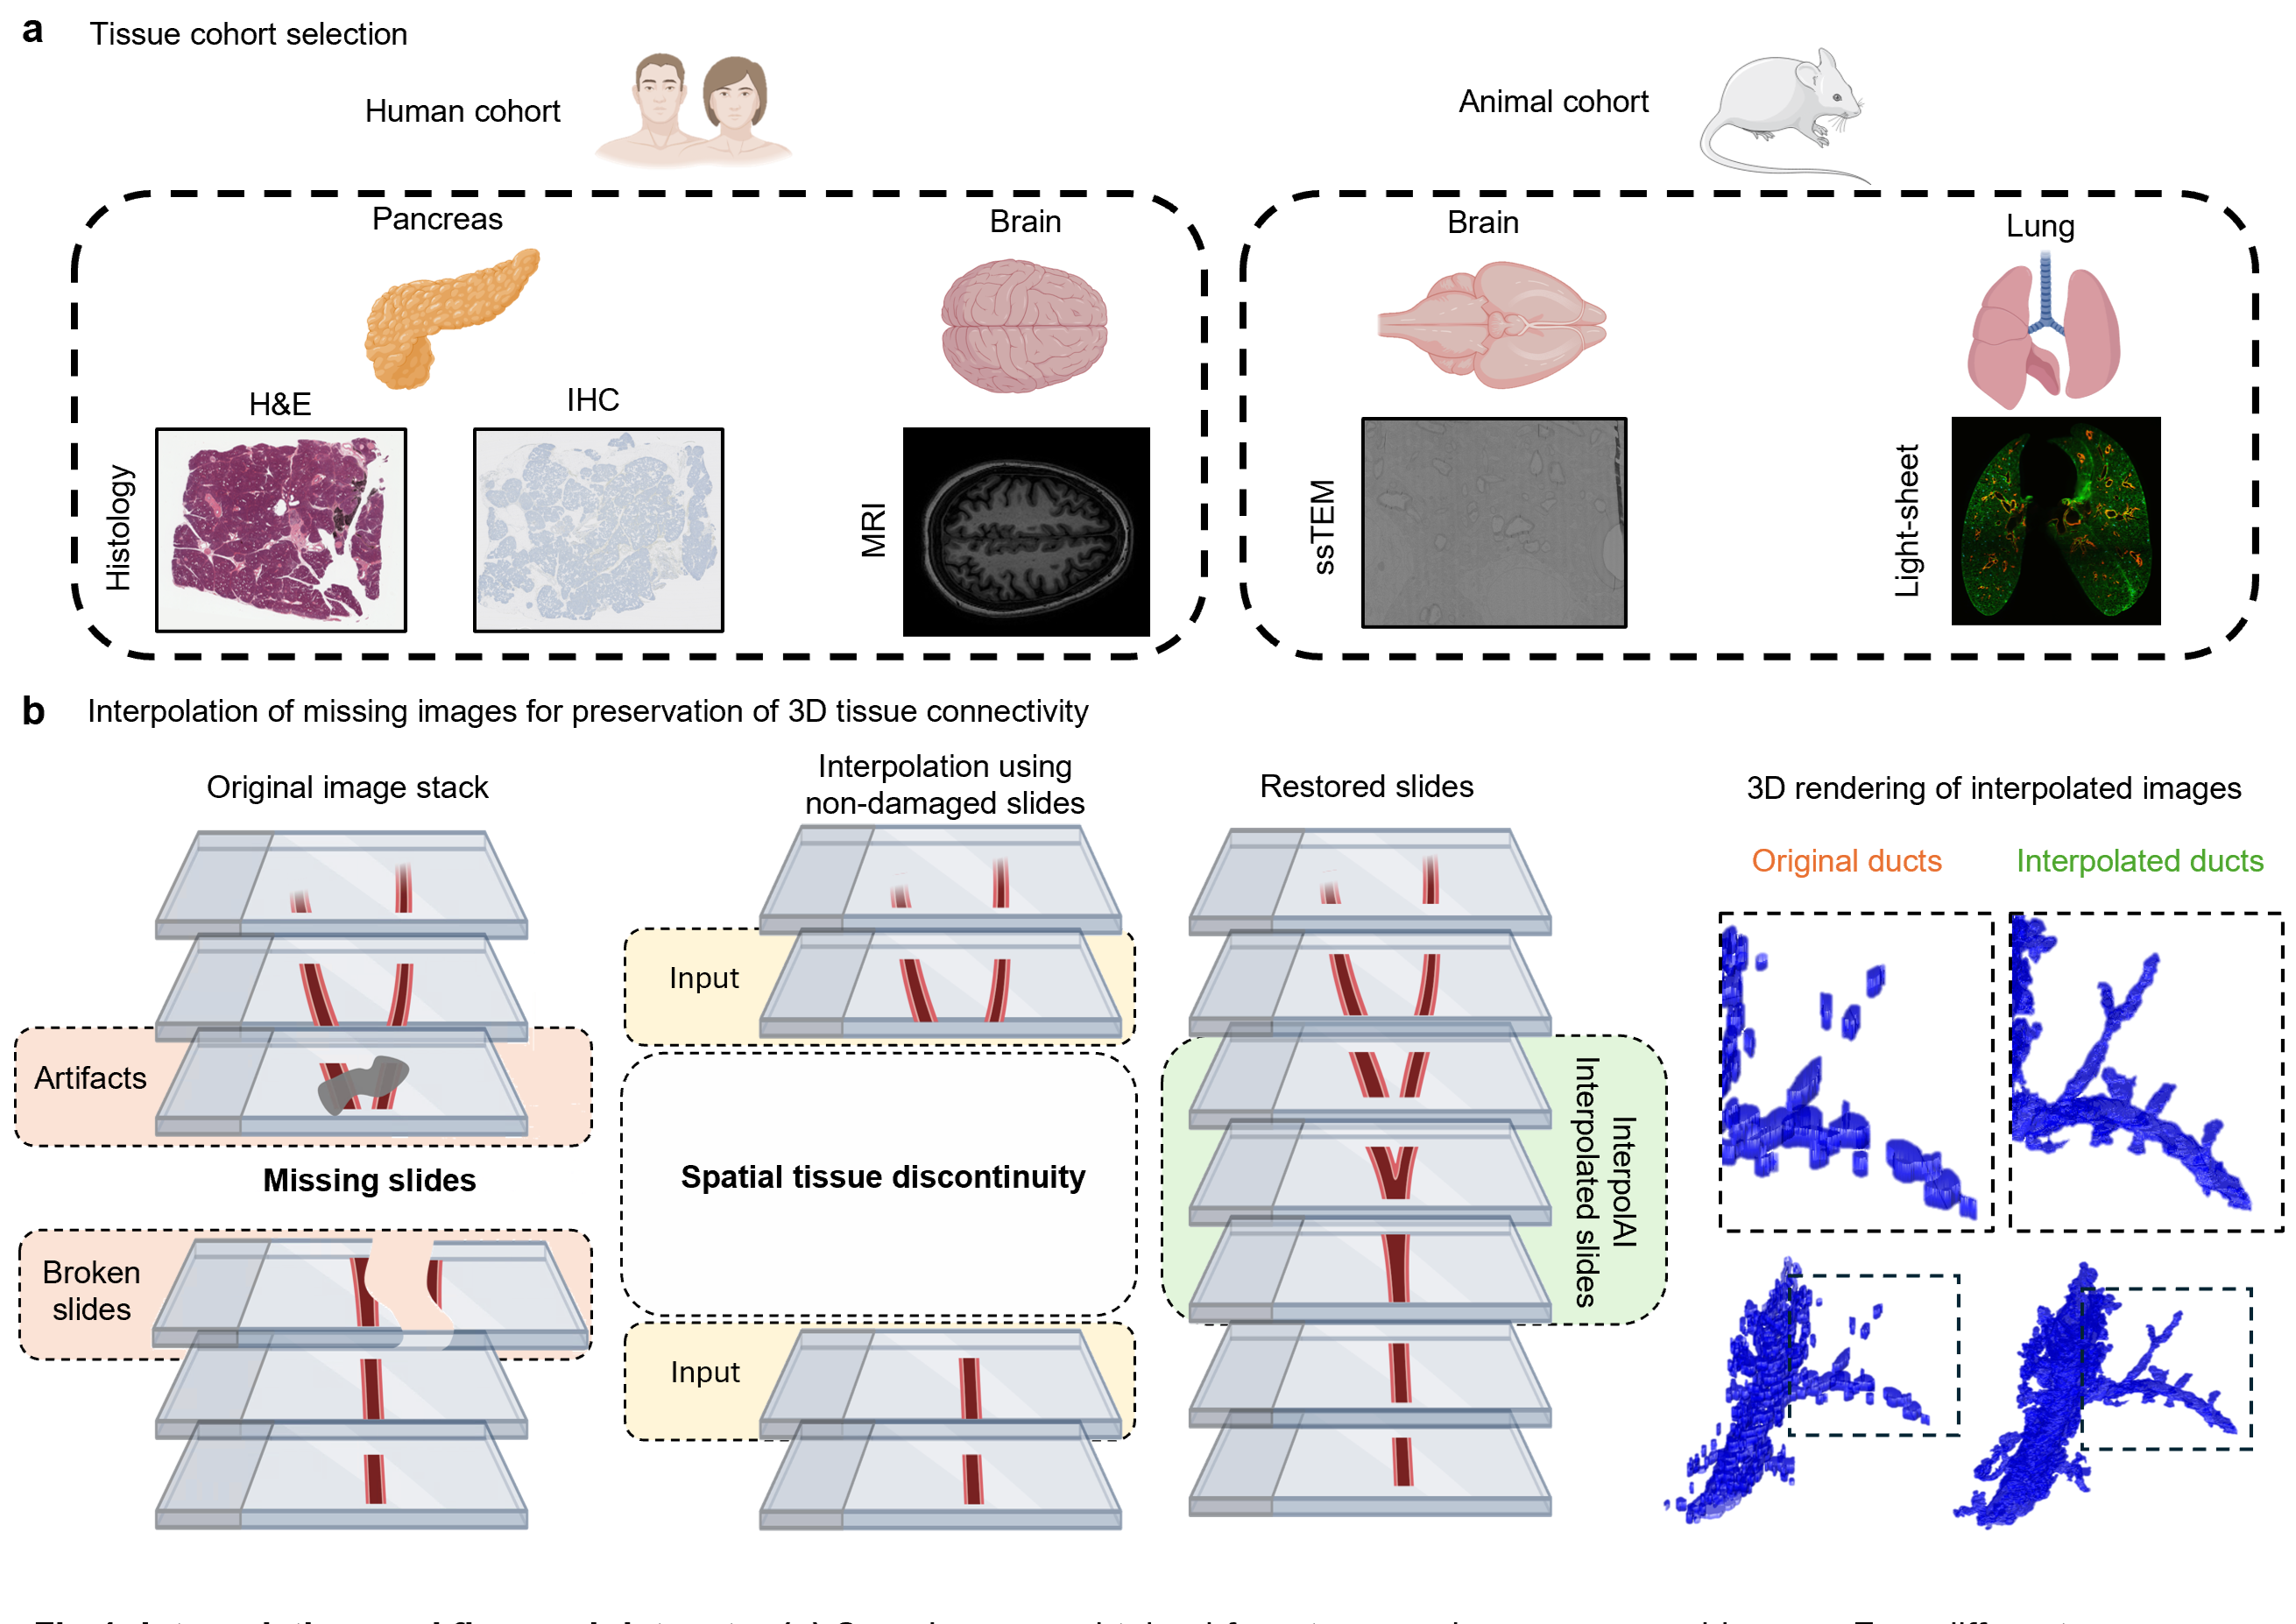
\includegraphics[width=1\textwidth,height=0.85\textheight,keepaspectratio,clip,page=1]{figures/chapter6/fig_1.png}
            \captionsetup{font=small}
            \caption{\textbf{Interpolation workflow and test datasets.} a, Samples were obtained from two species, mouse and human. Four different organs were analyzed: human pancreas, human brain, mouse brain and mouse lung. Five imaging modalities were tested: H\&E-stained histological slides, IHC stained histological slides, MRI, serial ssTEM slides and combined tissue clearing and light-sheet microscopy. b, Aligned slides are manually searched through to identify missing or damaged slides, and damaged slides are removed from the stack of slides. InterpolAI missing slides as inputs to recreate slides that were stained differently, missing or damaged, resulting in a uniform stack of slides. Using CODA, slides are segmented into labeled tissue masks, with each label representing a different microanatomical structure in the slide, which is then used to recreate and visualize microanatomical 3D structures in the tissue sample. Illustrations created using BioRender.com.}
            \label{chapter6_fig1}
        \end{center}
    \end{figure}
    
    % \begin{figure}[h!]
    %     \ContinuedFloat
    %     \captionsetup{font=small}
    %     \caption[]{}
    % \end{figure}
    
    \section{InterpolAI interpolation for stacks of histological slides}
    We tested the ability of InterpolAI to interpolate WSIs within a stack of histological images from human pancreatic tissue samples. Histological slides are often lost or damaged due to defects created during tissue sectioning or improper storage and documentation\cite{}.13,14 The ability of InterpolAI to interpolate slides was compared to XVFI, a state-of-the-art optical flow based interpolation method, and linear interpolation of the same slides and then compared to the corresponding authentic slide (Fig. \ref{chapter6_fig2})\cite{leng2013a,upchurch2017a,liu2011a,blu2004a}. To qualitatively compare the interpolated slides, two regions of interest (ROI’s) from the 101 serially sectioned and H\&E stained human pancreas dataset were selected based on the anatomical structures present. These ROIs had a total of eight tissue components, including islets of Langerhans, ductal epithelium, blood vessels, fat, acini, ECM, whitespace, and PanIN (precursor) lesions. Two images were selected one every 8 images (denoted skip 7) of the original stack of authentic images, and the missing 7 images were interpolated (Fig. \ref{chapter6_fig2}a). Interpolated images were compared against their respective authentic images (Fig. \ref{chapter6_fig2}, b and c).
    Due to their complex branching character within the first ROI, which represent a 3D imaging challenge, we examined ducts and blood vessels (Fig. \ref{chapter6_fig2}b). Comparison with authentic image of the duct showed that the damage was fixed by InterpolAI interpolation (top row, top arrow, Fig. \ref{chapter6_fig2}b). In contrast, the epithelium layer of the duct showed significant noise in the linearly interpolated image due to pixel averaging (top row, bottom arrowhead, Fig. \ref{chapter6_fig2}b). This caused overlay artifacts that were absent in InterpolAI, which tracked pixel “movements” using optical flow for a sharper image. Linear interpolation improperly replaced the damaged areas with acinus-like material instead of whitespace in the authentic slide (top row, top arrowhead, Fig. \ref{chapter6_fig2}b). In contrast, InterpolAI successfully removed the damage and preserved the whitespace (top row, top arrow, Fig. \ref{chapter6_fig2}b). Similarly to InterpolAI, XVFI removed a significant amount of damage replacing it with whitespace, however some black damage artifacts remained (top row, top dashed arrow, Fig. \ref{chapter6_fig2}b). Unlike InterpolAI, XVFI also incorrectly generated hued acini structures within the whitespace it interpolated (top row, right dashed arrow, Fig. \ref{chapter6_fig2}b). Furthermore, InterpolAI preserved the central structure of the duct, whereas linear interpolation thinned and elongated the lumen (top row, middle arrowhead, Fig. \ref{chapter6_fig2}b). 
    The superiority of InterpolAI over linear interpolation was further observed in blood vessels (bottom row, bottom arrowhead, Fig. \ref{chapter6_fig2}b). Overlay artifacts were present throughout the entire structure of the blood vessel when using linear interpolation (bottom arrow, Fig. \ref{chapter6_fig2}b). Unlike InterpolAI, linear interpolation could not preserve the structure of the blood vessel (Fig. \ref{chapter6_fig2}b). Linear interpolation also incorrectly generated regions of fat that were absent in the authentic images (bottom row, top arrowhead, Fig. \ref{chapter6_fig2}b). While XVFI accurately interpolated the structure of the blood vessel, the sharpness of the interpolated image was degraded compared to the authentic and InterpolAI images, resulting in cells in the acini that looked blurred or absent (bottom row, Fig. \ref{chapter6_fig2}b). 
    In the second ROI, chosen because it was enriched in ducts, fat, and islets, linear interpolation created an artificial shadow in the duct lumen (top row, top arrowhead, Fig. \ref{chapter6_fig2}c). XVFI accurately interpolated the structure of the duct but again was unable to interpolate cellular information, specifically epithelial cells lining the duct.  XVFI created a purple hued band that lacked cell nuclei around the lumen of the duct (top row, dashed arrows, Fig. \ref{chapter6_fig2}c and inset zoom-in).  In contrast, InterpolAI accurately interpolated the duct, while retaining cellular information (top row, Fig. \ref{chapter6_fig2}c and inset zoom-in). Other key structures included fat and islets, which were typically presented as small and faint morphologies (bottom row, Fig. \ref{chapter6_fig2}c). The authentic slide contained 8 fat and 5 islets structures, however linear interpolated images showed shadows of fat where real fat was located (bottom row, top arrowhead, Fig. \ref{chapter6_fig2}c). Additionally, it generated non-existent fat (bottom row, bottom arrowhead Fig. \ref{chapter6_fig2}c). These fat shadows could be wrongly interpreted as islets, especially in regions where islets were present (bottom row Fig. \ref{chapter6_fig2}c). Although InterpolAI struggled with overlapping fat, it properly interpolated distinct fat without artifacts and could clearly distinguish islets from fat.
    Using CODA cell detection module, the total cell counts were computed for each of the interpolated H\&E images and compared to corresponding counts in authentic images. This cell count was repeated for each scenario of skipping 1, 3, and 7 slides (Fig. \ref{chapter6_fig2}d). Linear interpolation consistently generated images containing more cells than in the authentic images, as a result of overlay artifacts. XVFI was unable to interpolate cellular information and instead generated images that appeared blurred or out of focus, resulting in images displaying far fewer cells than the authentic images. While InterpolAI-interpolated images also generated more cells on average than in the authentic images, the percent error in cell count for the stack of InterpolAI-interpolated images was <5\% for each interpolation scenario. Linear interpolation resulted in a percent error in cell count >10\% and XVFI had a percent error in cell count >20\% for each interpolation scenario (Fig. \ref{chapter6_fig2}d). 
    Thirteen Haralick features (angular second moment, contrast, correlation, sum of squares variance, inverse difference moment, sum average, sum variance, difference variance, sum entropy, difference entropy, entropy, information measure of correlation 1, and information measure of correlation 2) were measured to evaluate the quality of interpolated images\cite{brynolfsson2017a,haralick1973a}. The results of each score were averaged for the different tested scenarios (authentic, InterpolAIskip1, InterpolAIskip3, InterpolAIskip7, linearskip1, linearskip3, linearskip7, XVFIskip1, XVFIskip3, and XVFIskip7) (Table S1.), which allowed for principal component analysis (PCA) to be carried out (Fig. \ref{chapter6_fig2}e). This analysis demonstrated that the InterpolAI-interpolated slides represented more closely the information in the authentic slides, even when skipping seven slides, as compared to linear interpolation and XVFI, which was the furthest from authentic images. The Euclidean distance of the 13 Haralick features between authentic and interpolated images was computed (Fig. \ref{chapter6_fig2}e). Even when skipping 7 slides, InterpolAI images were less than 1/2 the distance from authentic images for linearly interpolated images when skipping just 1 slide. When comparing independent interpolation scenarios between InterpolAI and XVFI, InterpolAI images were also <1/2 the distance of XVFI images to the authentic images.  
    Standard metrics, such as mean square error (MSE), structural similarity index measure (SSIM), peak signal-to-noise ratio (PSNR), Spearman correlation, Jaccard correlation, Sobel filter, and channel wise pixel-to-pixel intensity correlation could not quantify the (very visible) structural errors in the microanatomical features generated by linear interpolation (Fig. \ref{chapter6_fig2}, b and c). Acini, which are the dominant structure in the healthy pancreas, could easily be interpolated, resulting in similar metric values for linear and InterpolAI, since these metrics are less sensitive to small-pixel deviations compared to large-pixel deviations. We attempted masking acini to focus on microanatomical structures, but registration differences between images only highlighted alignment issues rather than interpolation quality.
    Validation with expert pathologists at the Johns Hopkins School of Medicine (GI division, Dept Pathology) was attempted to determine the authenticity of interpolated images. Initially, pathologists were unable to distinguish microanatomical differences between authentic and InterpolAI-generated images. Over time, pathologists distinguished interpolated from authentic images by their reduced damage artifacts.
    In sum, InterpolAI can accurately interpolate damaged or missing H\&E-stained histological images, which restores lost information in stacks of 2D images and, consequently, improves connectivity of 3D continuous microanatomical structures (see additional details below). Unlike linear interpolation, InterpolAI does not generate non-existent microanatomical structures, such as ducts or fat in pancreatic tissues, and preserves cellular information better than XVFI.

    \begin{figure}[p]
        \begin{center}
            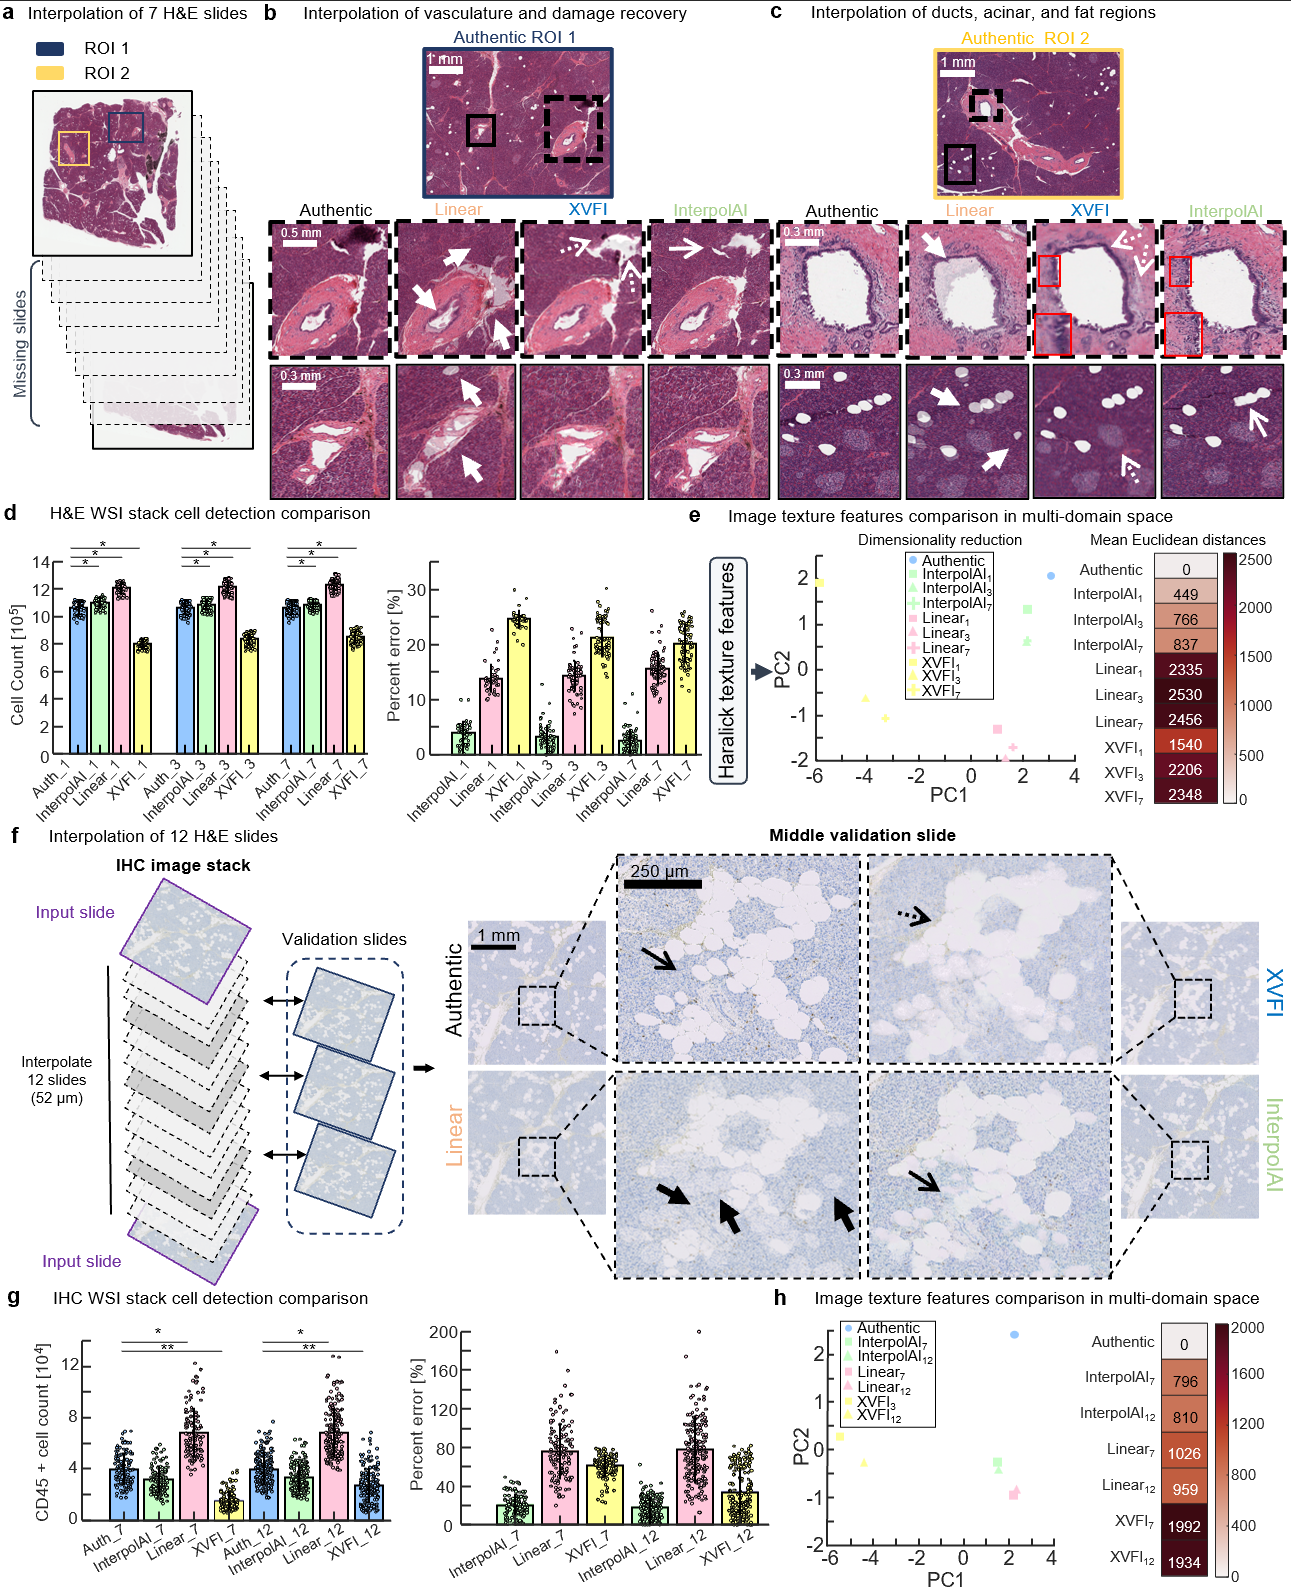
\includegraphics[width=1\textwidth,height=0.85\textheight,keepaspectratio,clip,page=1]{figures/chapter6/fig_2.png}
            \captionsetup{font=small}
            \caption{\textbf{Comparison of linear, XVFI and InterpolAI interpolations for pancreatic histology image stacks.} a, ROI were selected from WSIs to include
            all microanatomical features (islets, ducts, vessels, fat, acini, ECM and PanIN).
            Slides were interpolated, skipping seven slides between adjacent sections,
            generating seven slides.}
            \label{chapter6_fig2}
        \end{center}
    \end{figure}
    
    \begin{figure}[h!]
        \ContinuedFloat
        \captionsetup{font=small}
        \caption[]{ b, ROI 1 shows a comparison of interpolated to
            the authentic ROI for the middle-interpolated image for ducts and vessels.
            Arrowheads show linear interpolation replacing damage with acini as opposed
            to whitespace, creating noise around the ducts, incorrectly generating fat
            and unable to preserve vessel structure. Dashed arrows show XVFI removed
            damage, kept some black damage artifacts and incorrectly generated hued acini
            within the interpolated whitespace. Arrow shows InterpolAI correctly restored
            whitespace. c, ROI 2 shows a comparison of interpolated to the authentic ROI for
            the middle-interpolated image for ducts, fat and vessels. Arrowheads show linear
            interpolation creates duct lumen and fat shadows resembling islets as well as
            nonexistent fat regions. Red boxes show XVFI was unable to interpolate cellular
            information unlike InterpolAI. Dashed arrows show XVFI created a purple hued
            band, lacking cell nuclei around the lumen of the duct. d, Cell counts comparison
            between authentic H\&E and interpolated images, and percentage error in cell
            counts. e, PCA of 13 Haralick features for authentic, and interpolated images for
            various numbers of skipped images. Mean Euclidean distance of interpolated
            images from authentic images based on 13 Haralick features. f, IHC slides were
            interpolated and compared to authentic slides for validation. Middle slide is
            compared with the interpolated images. Arrow shows InterpolAI preserves
            vessel structure, unlike linear interpolation, which was also unable to preserve
            fat domains such as XVFI (arrowheads and dashed arrow). g, Comparison of
            CD45+ cell counts in authentic images and interpolated images when skipping
            7 and 12 slides. h, PCA of 13 Haralick features for authentic and interpolated
            IHC images for various numbers of skipped images. Mean Euclidean distance
            of interpolated images from authentic images is based on 13 Haralick features.
            Error bars represent mean ± s.d. *P ≤ 0.05, **P ≤ 0.01, ***P ≤ 0.001, ****P ≤ 0.0001.
            Supplementary Table 2 for exact P values calculated via two-tailed Mann–
            Whitney U-test, mean and s.d.}
    \end{figure}
    
    \section{InterpolAI for immunohistochemistry (IHC) image stacks}
    To further demonstrate the ability of InterpolAI to interpolate histological WSIs, a second human pancreas sample was stained using immuno-histochemistry (IHC) for the leukocyte marker CD45. We note the substantial distance between input slides - 52μm - equivalent to omitting twelve successive 4-μm-thick sections (Fig. \ref{chapter6_fig2}f). The target images, for which authentic validation slides were available for comparison, are shaded in dark grey, while the missing slides between the input and target slides are shaded in light grey (Fig. \ref{chapter6_fig2}f). 
    We compared the middle-interpolated slide to the middle authentic validation slide using both linear and InterpolAI models (Fig. \ref{chapter6_fig2}f). In fat dense regions, linear interpolation artifacts were evident, while InterpolAI lacked such artifacts (arrow, Fig. \ref{chapter6_fig2}f). Additionally, whereas distinct cells were readily identified in the authentic image, the linearly interpolated image showed faintly stained cells covered with white hues resembling fat (right arrowhead, Fig. \ref{chapter6_fig2}f). Similarly, XVFI generated slides showed faded and blurred cells and did not accurately preserve the structure of fat regions, which lacked edges and resembled whitespace (dashed arrow, Fig. \ref{chapter6_fig2}f). In contrast, InterpolAI could interpolate distinct cells around the fat and preserved most of the ductal and ECM structures (arrow, Fig. \ref{chapter6_fig2}f), unlike the linear interpolation (left arrowhead, Fig. \ref{chapter6_fig2}f).
    Using CODA, the total cell count of CD45 positive (CD45+) cells was determined for linear, XVFI, and InterpolAI interpolated images and compared to the cell counts in the authentic images, while skipping and interpolating 7 and 12 slides. Linear interpolation resulted in higher CD45+ cell counts than those in authentic slides. Conversely, XVFI interpolation resulted in cell counts far lower than those in the authentic slides. InterpolAI-interpolated slides resulted in lower cell counts than in the authentic slides, but most closely matched the cell count trend in authentic slides (Fig. \ref{chapter6_fig2}g). Linearly interpolated slides had the highest percent error in CD45+ cell count, reaching > 100\% for certain slides, followed by XVFI and InterpolAI interpolated slides, with a mean error of 22\% in cell count (Fig. \ref{chapter6_fig2}g).
    Thirteen Haralick texture features were evaluated when interpolating 7 and 12 slides. The results of each score were averaged for the different scenarios assessed (authentic, InterpolAIskip7, InterpolAIskip12, linearskip7, linearskip12, XVFIskip7, and XVFIskip12) (Table S1). PCA analysis showed that InterpolAI-interpolated slides more closely represented authentic slide information along principal component 1 and linear along component 2, while XVFI interpolated slides were the furthest away (Fig. \ref{chapter6_fig2}h). The measurement of the Euclidean distance between authentic and interpolated images demonstrated that InterpolAIskip12 more closely represented the authentic slides compared to both linearskip7 and XVFIskip7 (Fig. \ref{chapter6_fig2}h).
    In sum, by interpolating IHC-CD45 stained images and determining the difference in cell count between authentic and interpolated images, we show the ability of InterpolAI to interpolate not only multicellular structures in stacks of histological images, such as ducts and blood vessels, but also smaller features, such as individual cells. 
    
    
    
    \section{InterpolAI for stacks of light-sheet microscopy images}
    Next, we applied InterpolAI to interpolate images within a stack of light-sheet micrographs obtained from a cleared mouse lung. Light-sheet microscopy presents challenges, including photobleaching and light absorption, which may result in uneven illumination of the sample, and tissue movement during imaging, which can introduce further distortions. Pairs of images were selected skipping 7 images from the authentic stack (Fig. \ref{chapter6_fig3}a), and interpolated images were compared to their authentic counterparts.    
    Linear interpolation of light-sheet micrographs created artificial double-boundary lines around the bronchioles, which is biologically inaccurate (middle row, top arrowhead, Fig. \ref{chapter6_fig3}b) (bottom row, right arrowhead, Fig. \ref{chapter6_fig3}b). Similarly, XVFI created two additional bronchioles which do not exist in the authentic image inaccurate (middle row, dashed arrow, Fig. \ref{chapter6_fig3}b) and elongated the right edge of a bronchiole (bottom row, right dashed arrow, Fig. \ref{chapter6_fig3}b). In contrast, InterpolAI correctly interpolated images of bronchioles to accurately depict the structure observed in the authentic image (middle row, arrow, Fig. \ref{chapter6_fig3}b). The second row of zoom-ins shows that the authentic image suffers from artifacts of light absorption and photobleaching at the top left of the bronchiole, which cause bleeding of the green and red channels into the bronchiole (bottom row, left arrowhead, Fig. \ref{chapter6_fig3}b). Both linear interpolation and XVFI reduced these artifacts, but could not remove them entirely (bottom row, left arrowhead and left dashed arrow, Fig. \ref{chapter6_fig3}b), whereas InterpolAI removed the bleed of the red and green channels (bottom row, left arrow, Fig. \ref{chapter6_fig3}b). 
    Thirteen Haralick texture features were measured to compare authentic and interpolated images, when interpolating 1, 3, and 7 slides. The results for each score were averaged for the different comparisons (authentic, InterpolAIskip1, InterpolAIskip3, InterpolAIskip7, linearskip1, linearskip3, linearskip7, XVFIskip1, XVFIskip3, and XVFIskip7) (Table S1.), and shown in a PCA plane (Fig. \ref{chapter6_fig3}c). PCA analysis showed that linearly interpolated images were more closely representative of the authentic images compared to InterpolAI and XVFI interpolated images (Fig. \ref{chapter6_fig3}c).  Nevertheless, when considering the mean Euclidean distance, InterpolAI outperformed linear interpolation for each individual skip scenario and outperformed XVFI when skipping one and three slides (Fig. \ref{chapter6_fig3}c). The Euclidean distance by slide increased when interpolating using XVFI or interpolating linearly through the stack as opposed to InterpolAI, which remained consistent through the stack (Fig. \ref{chapter6_fig3}d).
    In sum, InterpolAI can interpolate stacks of light-sheet images to reduce photobleaching and light absorption artifacts present in the authentic images, better than XVFI and linear interpolation. Elimination of such artifacts allows for more accurate 3D reconstructions of tissue samples.

    \begin{figure}[!htb] 
        \begin{center}
            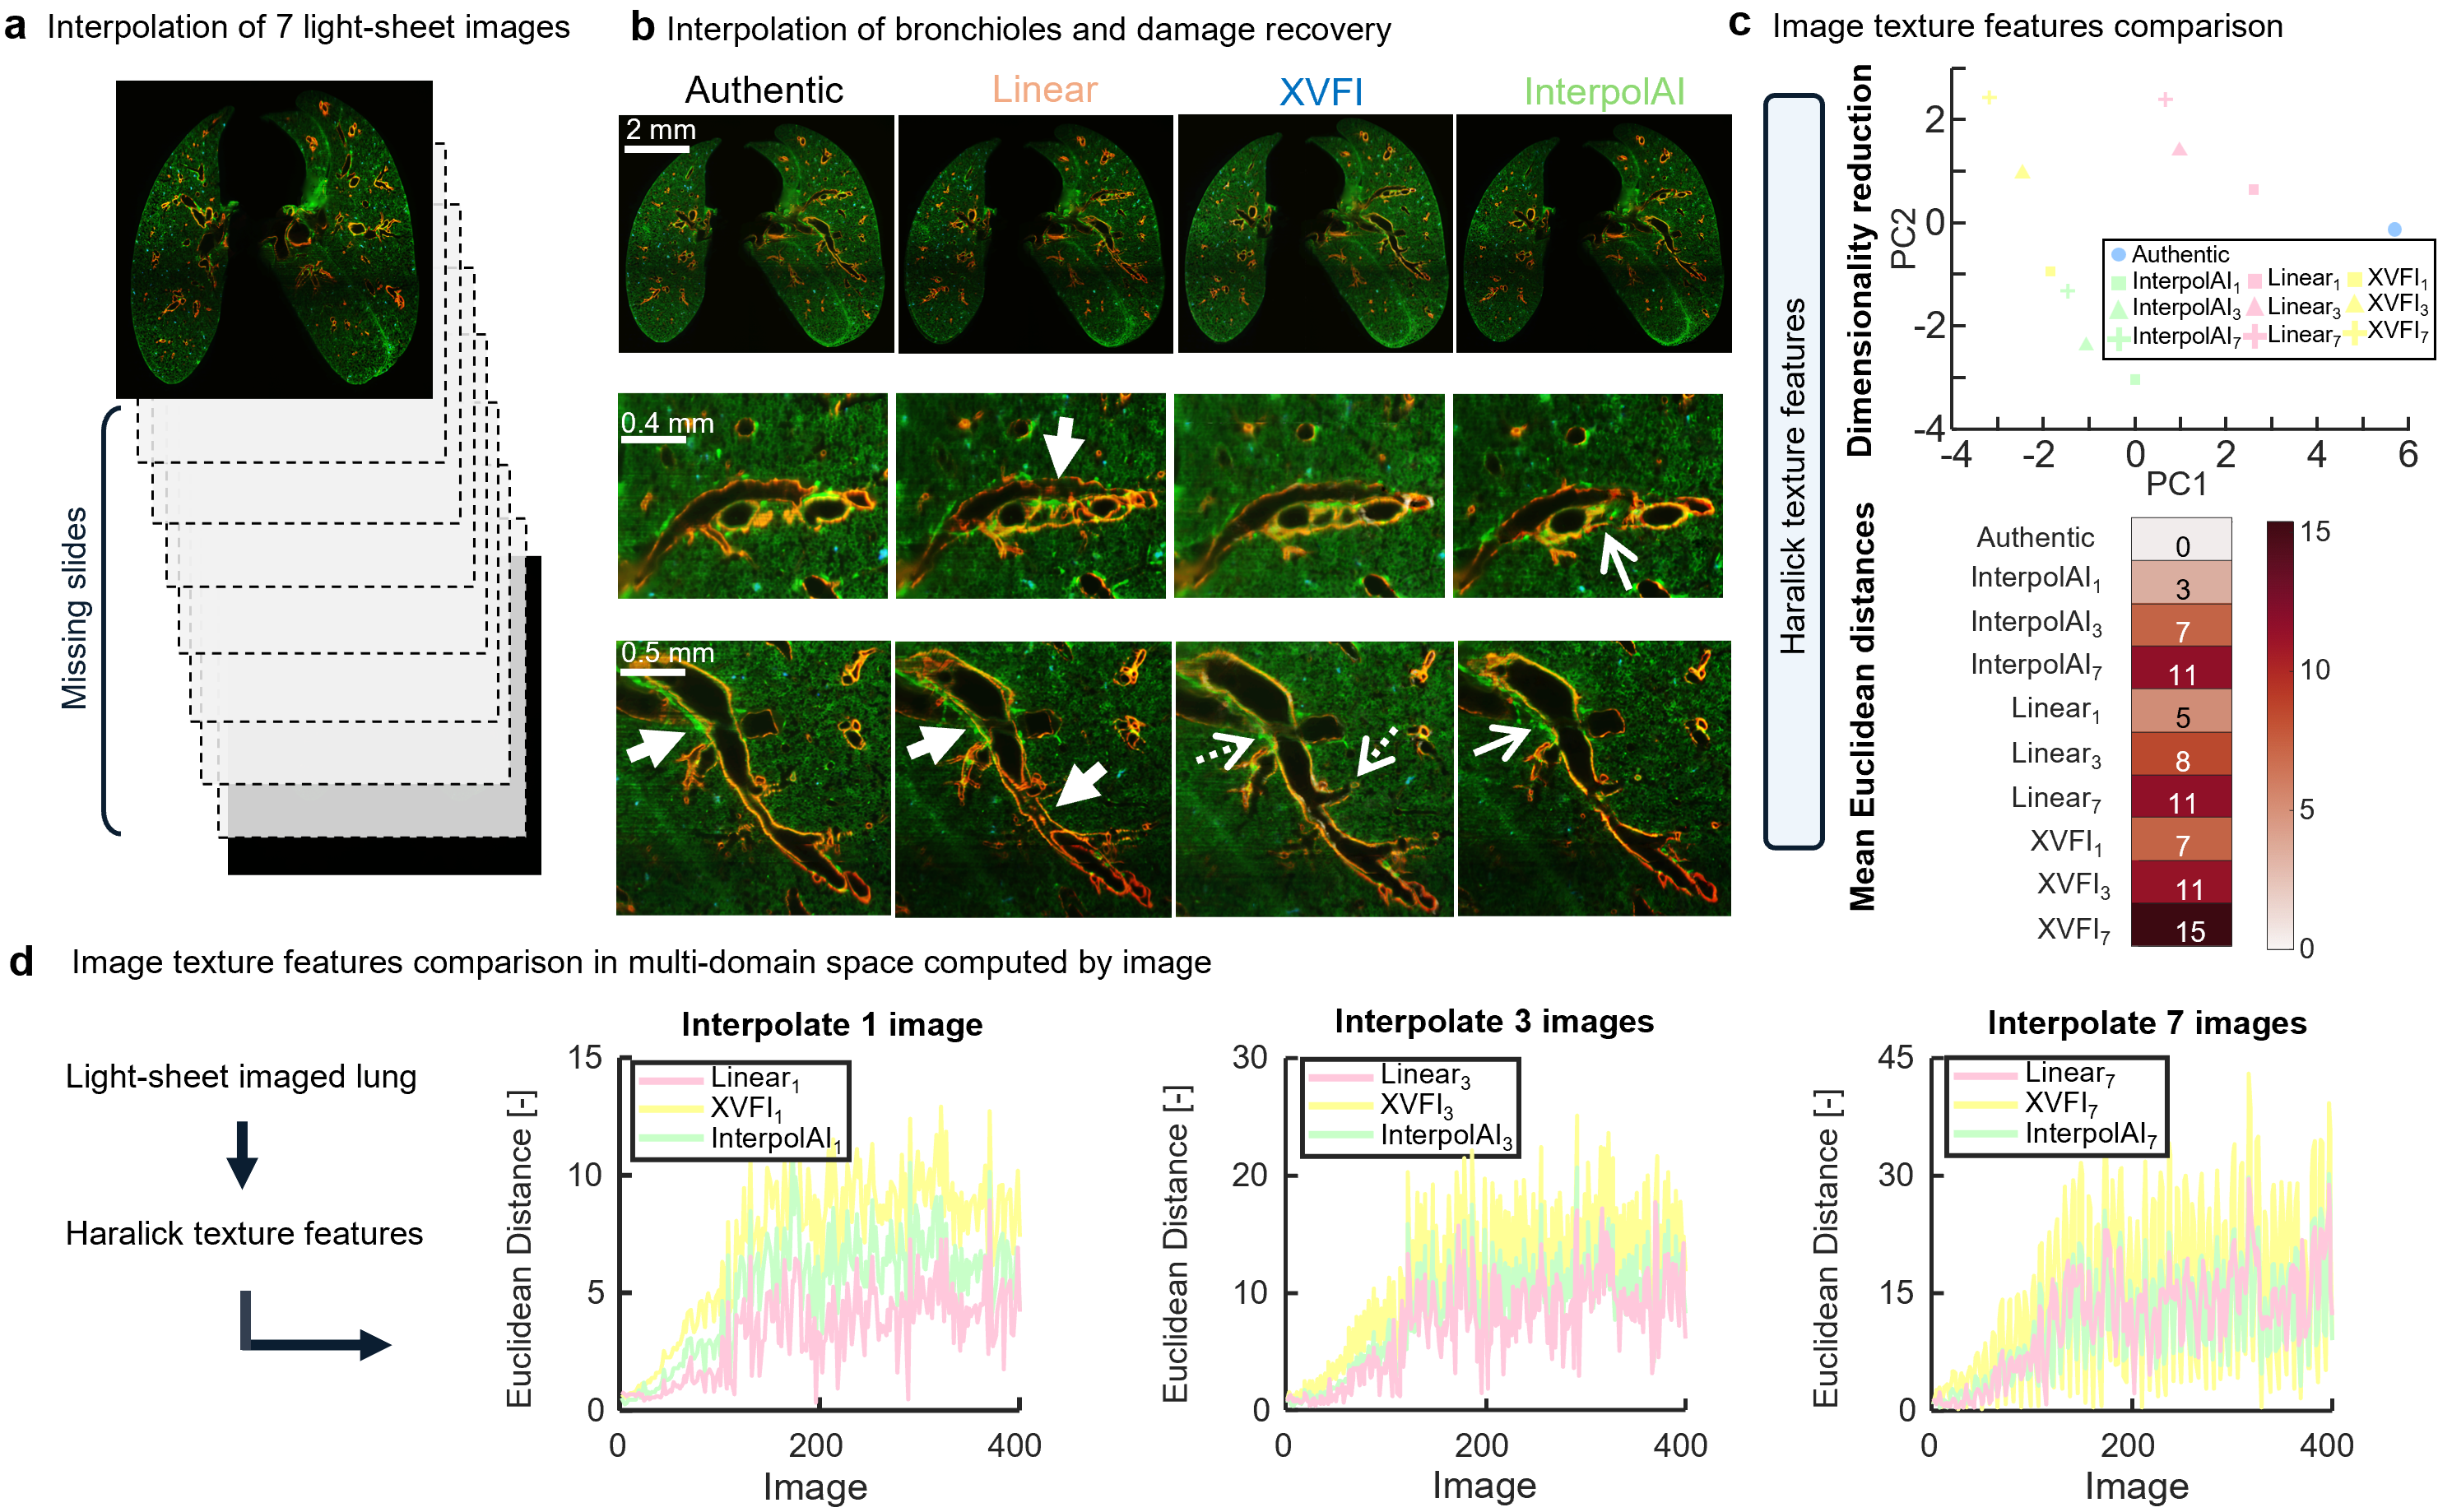
\includegraphics[width=1\textwidth,height=0.85\textheight,keepaspectratio]{figures/chapter6/fig_3.png}
            \captionsetup{font=small}
            \caption{\textbf{InterpolAI interpolation for stacks of MRI and light-sheet microscopy
            images.} a, Tissue-cleared light-sheet images were interpolated skipping seven
            slides between adjacent sections, thereby generating seven slides. b, Qualitative
            comparison of linear, XVFI and InterpolAI interpolations to the authentic image
            for the middle-interpolated light-sheet image (image 4). Arrowhead shows
            linear interpolation creates double boundary lines around bronchioles. In the
            second row, the arrowhead shows photobleaching in authentic reduced by linear
            interpolation and completely removed by InterpolAI (arrow). Dashed arrow
            shows XVFI reduced photobleaching but did not remove it. Second dashed
            arrow shows XVFI elongated the right edge of a bronchiole. c, PCA of 13 Haralick
            features for authentic, linear, XVFI and InterpolAI-interpolated light-sheet
            images for various numbers of skipped light-sheet images. Mean Euclidean
            distance of interpolated images from authentic images based on 13 Haralick
            features. d, Euclidean distance by slide of interpolated images from authentic
            images based on 13 Haralick features for various numbers of skipped lightsheet
            images.}
            \label{chapter6_fig3}
        \end{center}
    \end{figure}
    
    % \begin{figure}[h!]
    %     \ContinuedFloat
    %     \captionsetup{font=small}
    %     \caption[]{ }
    % \end{figure}
    
    \section{InterpolAI interpolation and restoration of ssTEM images}
    A stack of serial section transmission electron micrographs (ssTEM) of the mouse brain was used to show our ability to interpolate not only histological sections (Fig. \ref{chapter6_fig4}a). The authentic tiles shown Fig. \ref{chapter6_fig4}a represent a 2000x3500 pixel tile of the authentic whole slide image. Thick irregular black lines were observed across most of the slides in the authentic stack of images, which correspond to damage caused by unavoidable tissue tear during processing of thin sections (left column, arrows, Fig. \ref{chapter6_fig4}b). For a randomly selected subset of 100 consecutive slides from a stack of the >13,000 ssTEM slides, we found that >70\% were damaged, many of them containing >1 damaged region. Additionally, fainter grey lines were observed, going horizontally across the authentic images, which are artifacts of image stitching (top row, bound by red box Fig. \ref{chapter6_fig4}b). 
    Interpolation between two undamaged ssTEM slides using InterpolAI removed the damage to the slides while preserving their microanatomical structures, but also significantly reduce stitching artifacts (right column, Fig. \ref{chapter6_fig4}b).
    Thirteen Haralick features were measured for the authentic and interpolated images when interpolating 1, 3, and 7 slides. The results of each score were averaged for the different tested scenarios (authentic, InterpolAIskip1, InterpolAIskip3, InterpolAIskip7, linearskip1, linearskip3, linearskip7, XVFIskip1, XVFIskip3, and XVFIskip7) (Table S1). PCA showed that InterpolAI-interpolated slides more closely represented authentic slide information along principal component 2, while linear along component 1, and XVFI being the furthest away (Fig. \ref{chapter6_fig4}c). The short Euclidean distance between authentic and interpolated images suggests that InterpolAIskip1 more closely represents the authentic than linearskip1 and XVFIskip1 and similarly for the instance of skipping 3 and 7 slides (Fig. \ref{chapter6_fig4}c).
    In sum, we demonstrated the ability of InterpolAI to eliminate damage in ssTEM slides, allowing for more accurate 3D reconstructions of neural structures by decreasing the loss in connectivity that arises due to the damage in individual 2D sections.

    \begin{figure}[!htb] 
      \centering
      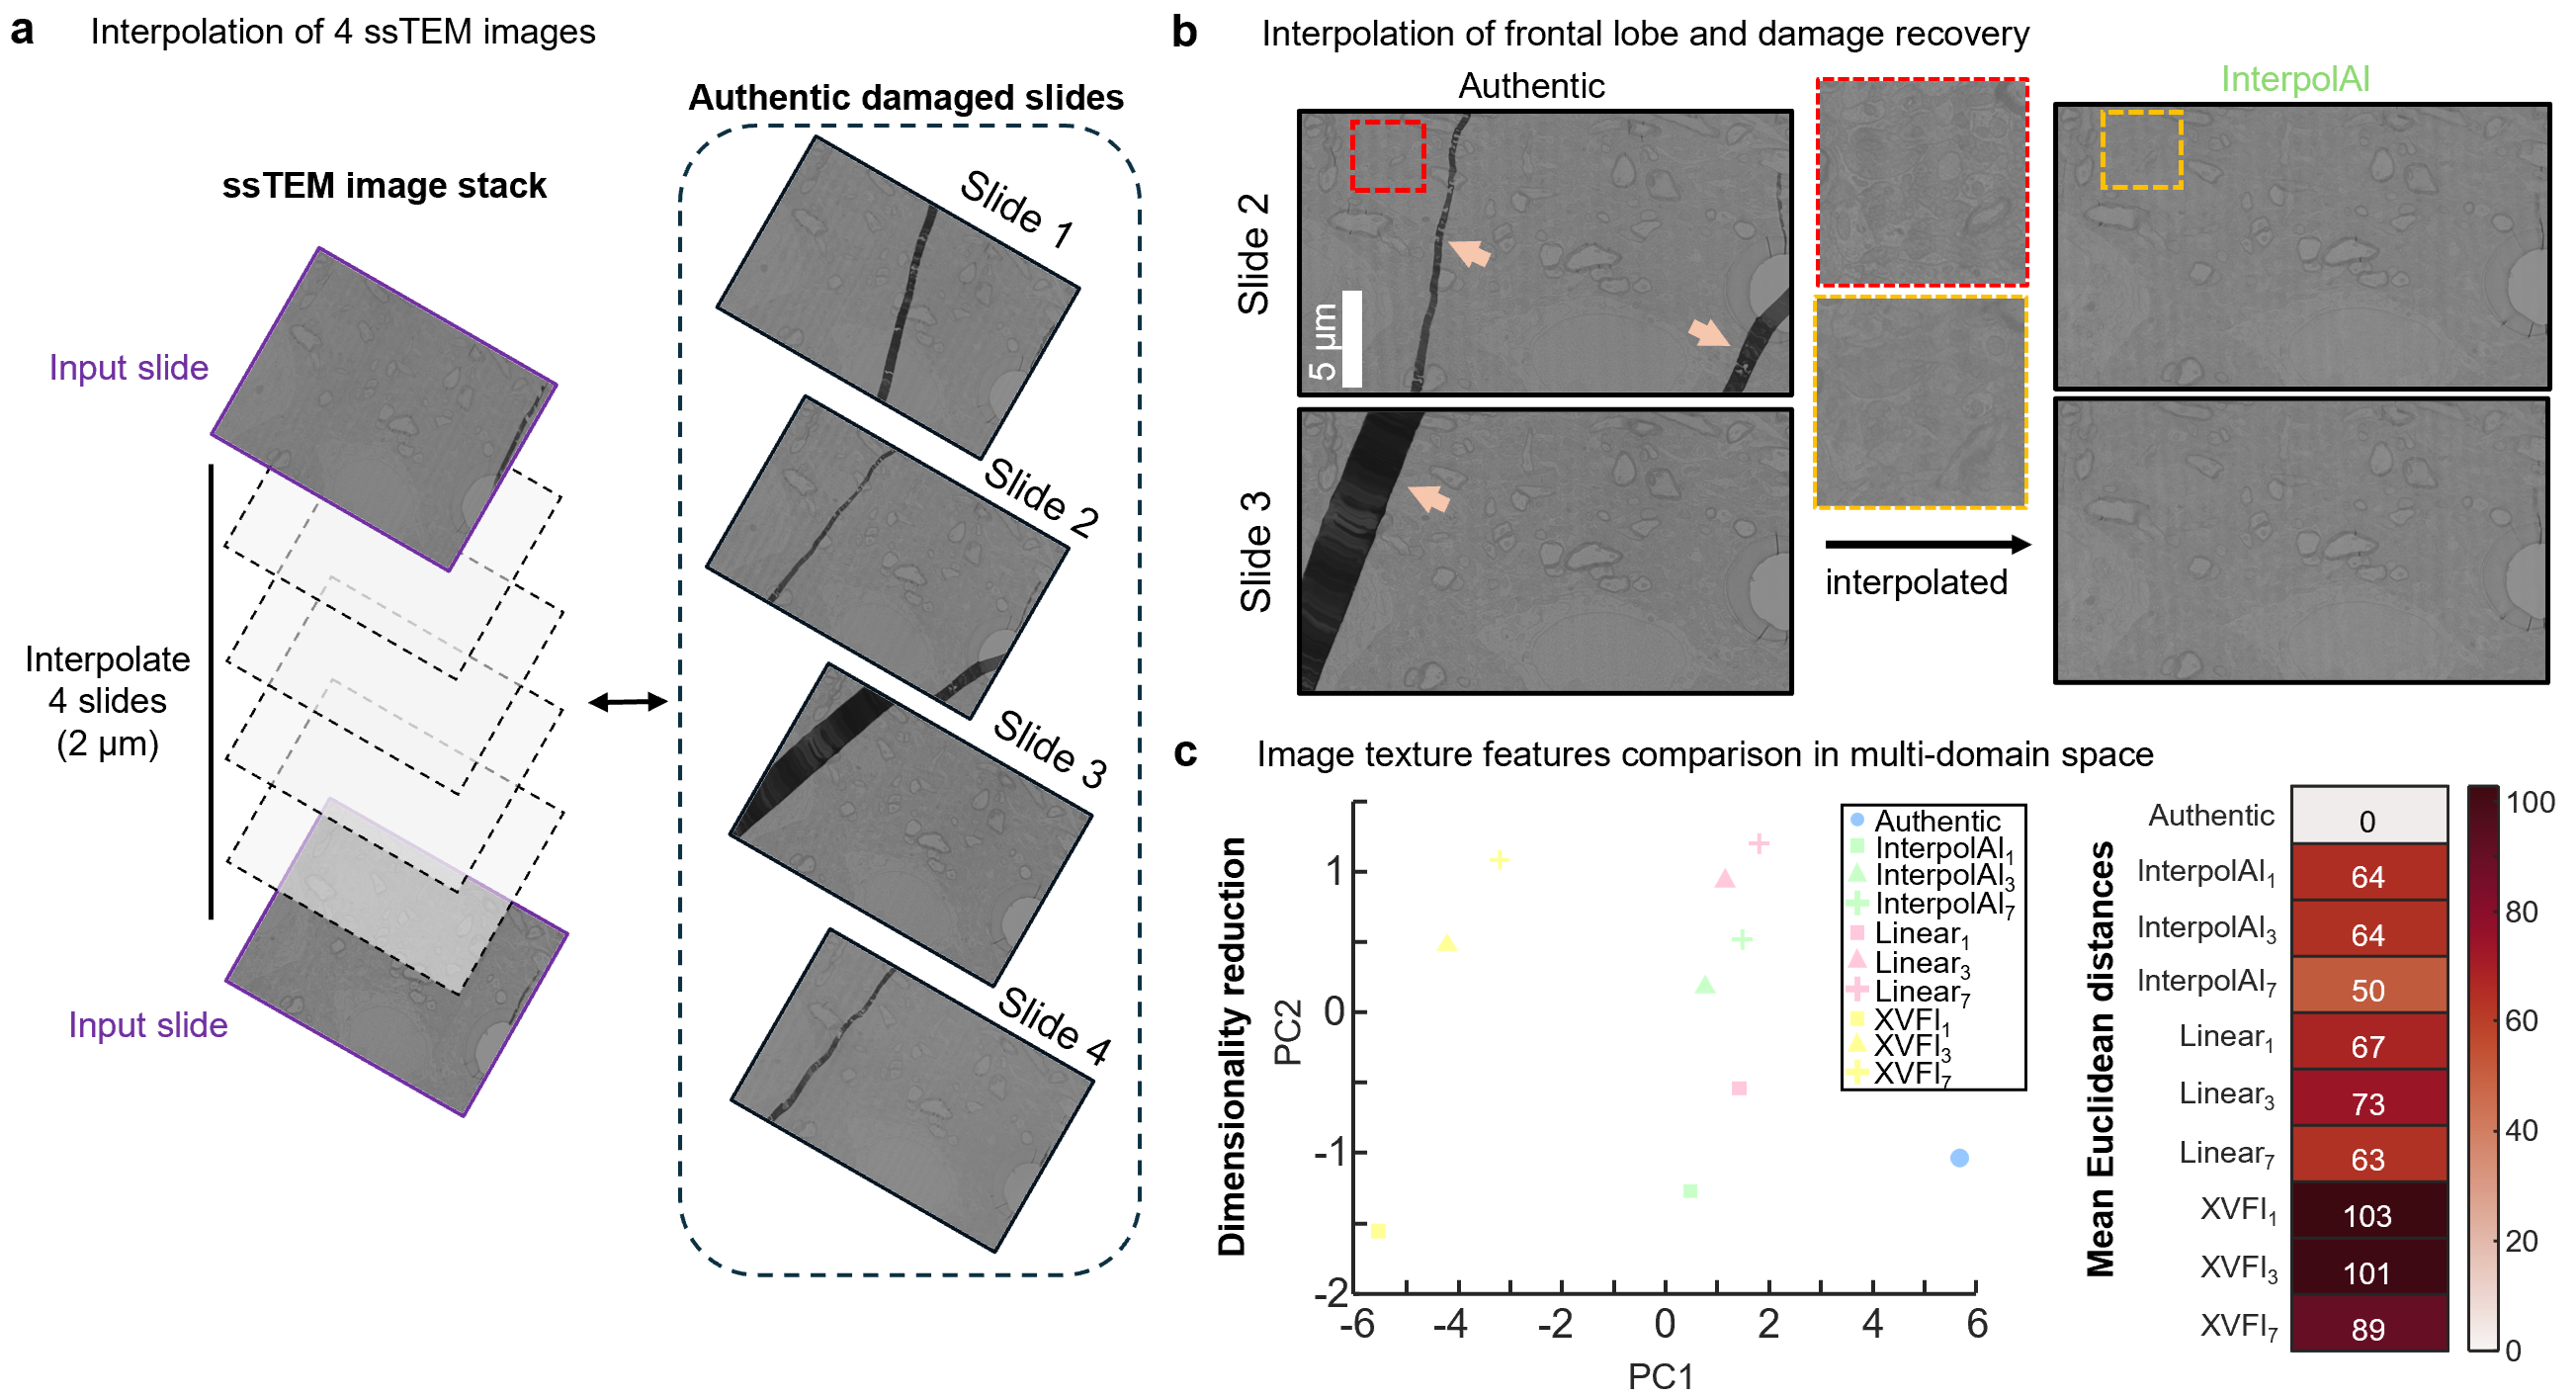
\includegraphics[width=\linewidth,                   height=0.85\textheight,                   keepaspectratio]{figures/chapter6/fig_4.png}
      \captionsetup{font=small}
      \caption{\textbf{InterpolAI interpolation for a stack of ssTEM images.}
               a, ssTEM slides were interpolated while skipping four slides
               between adjacent sections, thereby generating four slides.
               b, InterpolAI interpolation of mouse brain ssTEM slides to
               remove damage from slides (arrowheads) and reduce stitching
               artifacts (red box).
               c, PCA of 13 Haralick features for authentic, linear, XVFI and
               InterpolAI-interpolated ssTEM images for various skipped images.
               Mean Euclidean distance of interpolated images from authentic
               images based on 13 Haralick features.}
      \label{chapter6_fig4}
    \end{figure}
    
    % \begin{figure}[h!]
    %     \ContinuedFloat
    %     \captionsetup{font=small}
    %     \caption[]{ }
    % \end{figure}
    
    \section{InterpolAI interpolation for stacks of MRI images}
    To assess the ability of InterpolAI to interpolate low-resolution biomedical images, we interpolated images within stacks of MRI images (1mm x 1mm x 1mm). MRI imaging faces inherent limitations, such as susceptibility to motion artifacts due to prolonged scan times leading to patient discomfort and potential for signal loss due to magnetic field in homogeneities that can impact the quality of acquired images. Pairs of images were selected one every 8 images (skip 7) of the original stack of authentic images, and the missing 7 images were interpolated (Fig. \ref{chapter6_fig3}a). Interpolated images were validated against their respective authentic images (Fig. \ref{chapter6_fig3}b).
    Linear interpolation of MRI images caused band artifacts around the boundary of the soft tissue, unlike XVFI and InterpolAI (middle row, Fig. \ref{chapter6_fig5}b). However, as a result of thicker slices obtained during MRI imaging (1mm), InterpolAI could not always accurately interpolate large structural changes in soft tissue structures that occur when skipping 7 images (= 8mm) (bottom row, Fig. \ref{chapter6_fig5}b). Nevertheless, linear interpolation created structures what resembles a grey smudge with significant overlay artifacts, while XVFI created a faint and inaccurate structure (bottom row, Fig. \ref{chapter6_fig5}b), unlike InterpolAI. 
    Thirteen Haralick texture features were measured to compare authentic and interpolated MRI images, when interpolating 1, 3, and 7 slides. The results for each score were averaged for the different comparisons (Table S1), and shown in a principal component analysis (PCA) plane (Fig. \ref{chapter6_fig5}c). InterpolAI-interpolated slides represented more closely the information in the authentic slides, even when skipping seven slides, compared to linear interpolation and XVFI, which was the furthest. The averaged values were also used to compute the Euclidean distance between authentic and interpolated images (Fig. \ref{chapter6_fig5}c). Skipping seven slides, InterpolAI-interpolated slides were less than 1/2 the Euclidean distance between the authentic slides and the linearly or XVFI interpolated slides when skipping only one slide. The Euclidean distance by slide further emphasizes the superiority of InterpolAI over linear interpolation as the Euclidean distance increased when progressing through the stack of slides and interpolating linearly as opposed to InterpolAI (Fig. \ref{chapter6_fig5}d). 
    We demonstrated the ability of InterpolAI to interpolate low-resolution MRI images more accurately than linear and XVFI interpolations. InterpolAI reduces motion artifacts in MRI images, whereas linear interpolation exaggerates these artifacts, which result in band artifacts. Elimination of such artifacts allows for improved 3D reconstructions of whole organ structures. However, shorter interpolation distances might be required to account for large structural changes that occur as a result of the low z-resolution of MRI.
    
    \begin{figure}[!htb] 
      \centering
      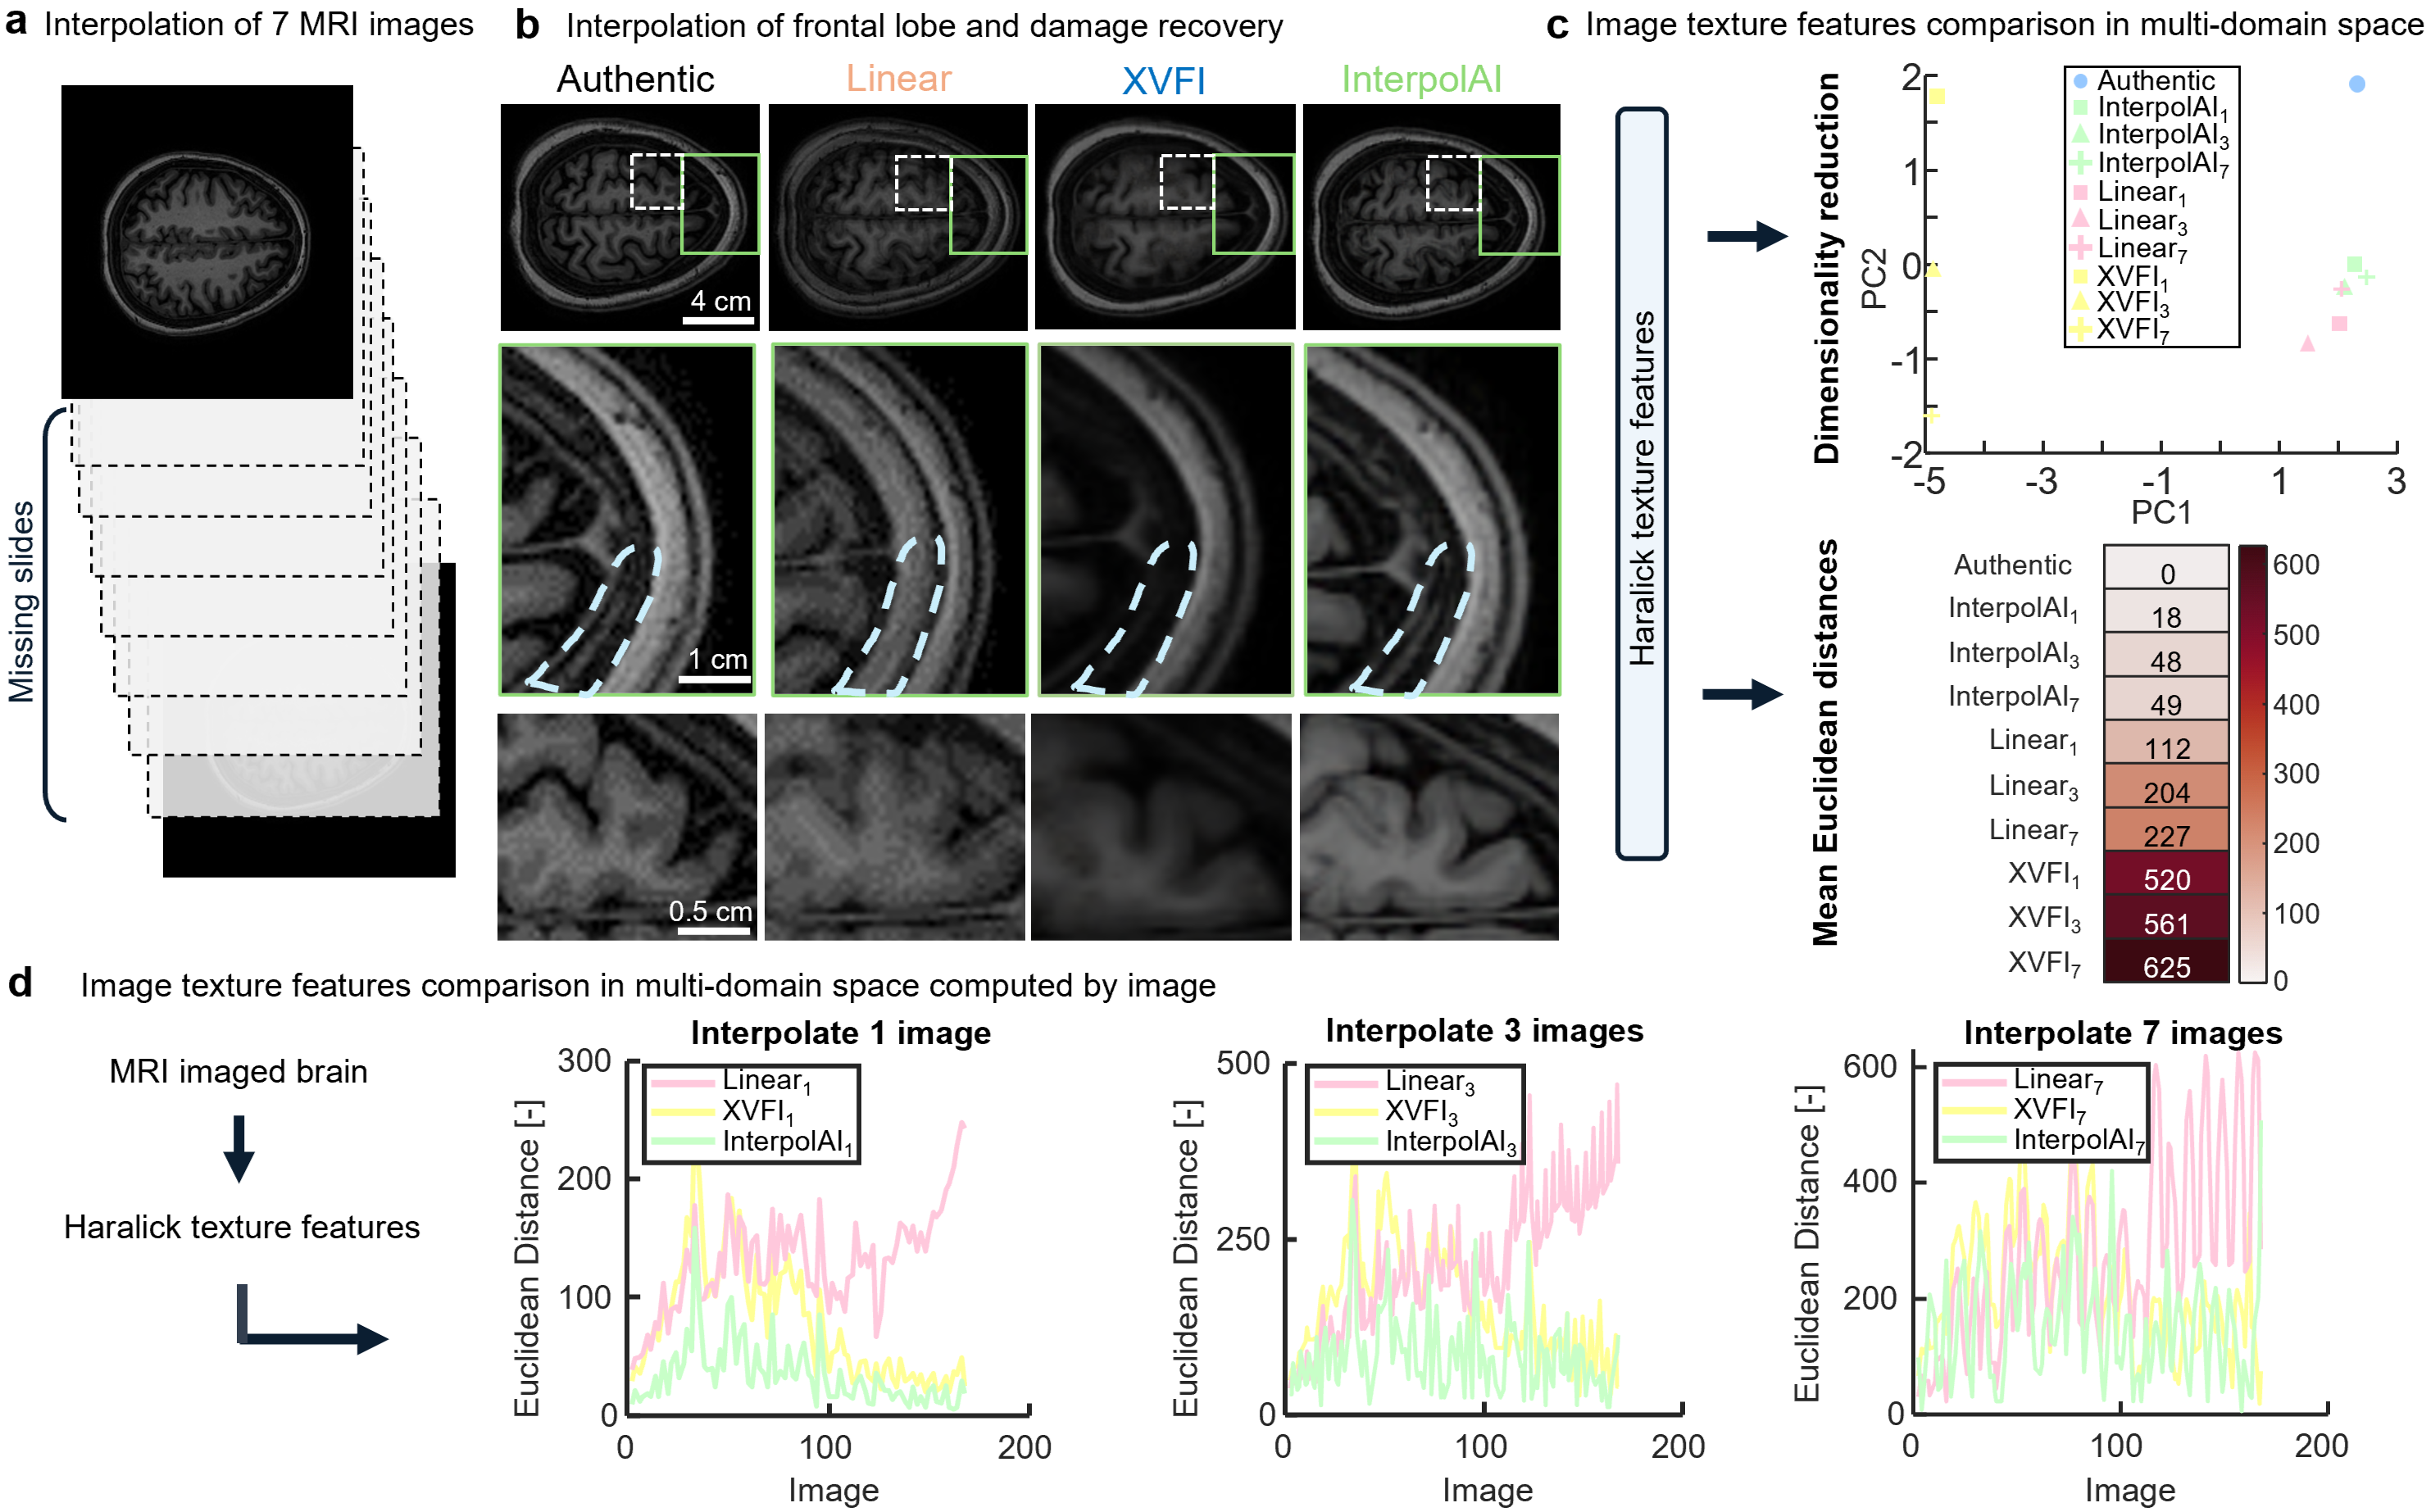
\includegraphics[width=\linewidth,                   height=0.85\textheight,                   keepaspectratio]{figures/chapter6/fig_5.png}
      \captionsetup{font=small}
      \caption{\textbf{InterpolAI interpolation for a stack of MRI images.} a, MRI images were
        interpolated while skipping seven slides between adjacent sections, thereby
        generating seven slides. b, Qualitative comparison of linear, XVFI and InterpolAI
        interpolation to the authentic image for the middle-interpolated MRI (image 4).
        The circled region shows linear interpolation creates band artifacts, unlike XVFI
        and InterpolAI. c, PCA of 13 Haralick features for authentic, linear, XVFI and
        InterpolAI-interpolated MRI images for various numbers of skipped images.
        Mean Euclidean distance of interpolated images from authentic images based on
        13 Haralick features. d, Euclidean distance by slide of interpolated images from
        authentic images based on 13 Haralick features for various numbers of skipped
        MRI images.}
      \label{chapter6_fig5}
    \end{figure}
    
    % \begin{figure}[h!]
    %     \ContinuedFloat
    %     \captionsetup{font=small}
    %     \caption[]{ }
    % \end{figure}
    
    \section{3D reconstruction of InterpolAI-interpolated images}
    To demonstrate the application of InterpolAI to restore 3D images of microanatomical structures obtained from interpolated 2D images, InterpolAI interpolation was applied across different image modalities, including stacks of histological (H\&E and IHC), light-sheet, ssTEM, and MRI images. Sematic segmentation and subsequent concatenation of the 2D segmented images into a volume allowed visualization of microanatomical features in 3D.
    Using CODA, we reconstructed in 3D the epithelial duct from the pancreatic H\&E dataset (Fig. \ref{chapter6_fig6}a). The 3D reconstruction of the authentic volume skipping 7 images displays the loss in ductal connectivity resulting from the missing slides. Linear interpolation of the H\&E samples created a low-resolution 3D structure of the duct which was artificially blocky (i.e. not smooth), and did not preserve the branching morphology of the duct (yellow zoom-in, arrowhead, Fig. \ref{chapter6_fig6}a). Linear interpolation also generated ductal structures which in parts missed their ductal wall (green zoom-in, arrowhead, Fig. \ref{chapter6_fig6}a).  In contrast, InterpolAI and XVFI restored the microanatomical connectivity in the 3D reconstruction of the main and smaller branches of the duct, while also creating a smoother volume without noise propagation (Supplementary Video 1). Although structurally accurate, XVFI compromised the identification of cells in H\&E images as demonstrated in Fig. \ref{chapter6_fig2}d.   
    Tissue-cleared light-sheet images were separated by channel and used to reconstruct in 3D the bronchioles of a mouse lung (Fig. \ref{chapter6_fig6}b). The comparison of the authentic volume to a downsampled reconstruction of the authentic volume (skipping 7 images between adjacent z-planes) showed a loss in connectivity of the bronchioles in 3D as a result of the missing image scans. The use of all three interpolation methods to recover missing z-planes resulted in improved connectivity of the bronchioles in 3D (Fig. \ref{chapter6_fig6}b). The results in 3D matched those observed in 2D (Fig. \ref{chapter6_fig3}), where all three interpolation methods were comparable in performance as demonstrated through 13 Haralick texture features.   
    Next, segmented ssTEM images were interpolated using linear, XVFI, and InterpolAI interpolation to reconstruct in 3D the synapses of the mouse brain. A qualitative assessment between the authentic volume and downsampled recreation of the authentic volume (skipping 7 images between adjacent z-planes) shows the loss in synapse connectivity (Fig. \ref{chapter6_fig6}c). Linear interpolation to recover the missing z-planes results in the creation of a low-resolution volume with blocky structures (green zoom-in, arrowhead, Fig. \ref{chapter6_fig6}c). Similarly, XVFI created a low-resolution volume, although less blocky than linear interpolation. Additionally, XVFI generated connected synapses as opposed to distinct tubules seen in the authentic volume (green zoom-in, dashed arrows, Fig. \ref{chapter6_fig6}c). Conversely, InterpolAI interpolation resulted in a higher resolution 3D volume, which resembled that of the authentic volume, and allowed for synapse connectivity to be restored (Supplementary Video 2).
    Finally, CODA was used to reconstruct a whole human brain in 3D using the stack of MRI images. A comparison of the reconstructed authentic volume to the authentic volume skipping 7 images showed how connectivity was lost as a result of the missing images. The reconstructed authentic volume skipping 7 images also lacked the topographical structure of the brain seen in the authentic volume, replacing it with single planes of information (Fig. \ref{chapter6_fig6}d). Using linear interpolation to recover the missing or damaged scans resulted in increased edges, which resembled objects extruding abnormally out of the brain. This is especially evident around the base of the brain where the brain stem protrudes and at the top of the brain towards the skull cap (green zoom-in, arrowhead, Fig. \ref{chapter6_fig6}d). Linear interpolation also generated a biologically inaccurate topography of the brain (yellow zoom-in, arrowhead, Fig. \ref{chapter6_fig6}d). XVFI generated a volume accurate in topography but failed to interpolate branching structures in the brain, specifically the brain stem (green zoom-in, dashed arrow, Fig. \ref{chapter6_fig6}d). When interpolating images using InterpolAI, the 3D reconstructed volume resembled more closely that of the authentic one, with accurate indentations and topography around the surface of the brain and even accurate reconstruction of the branching brain stem structure. 
    In sum, missing or damaged slides and images in biomedical image stacks cause significant loss in 3D spatial information, which hinders the accurate 3D reconstruction of microanatomical structures and whole organs from these image stacks. We demonstrate that linear interpolation is not sufficiently robust to recover the information lost in complex biomedical images, resulting in inaccurate 3D reconstructions. While XVFI interpolation preserves the structural connectivity of most microanatomical structures, it is limited in its ability to generate distinct and disjointed structures as seen with the ssTEM dataset. Additionally, as observed with the H\&E histology dataset XVFI cannot preserve the single-cell resolution found in H\&E images (Fig. \ref{chapter6_fig2}). In contrast, the optical flow-based model InterpolAI recovers more information to allow for 3D reconstructions that qualitatively and quantitively resemble their authentic counterparts.

    \begin{figure}[p] 
      \centering
      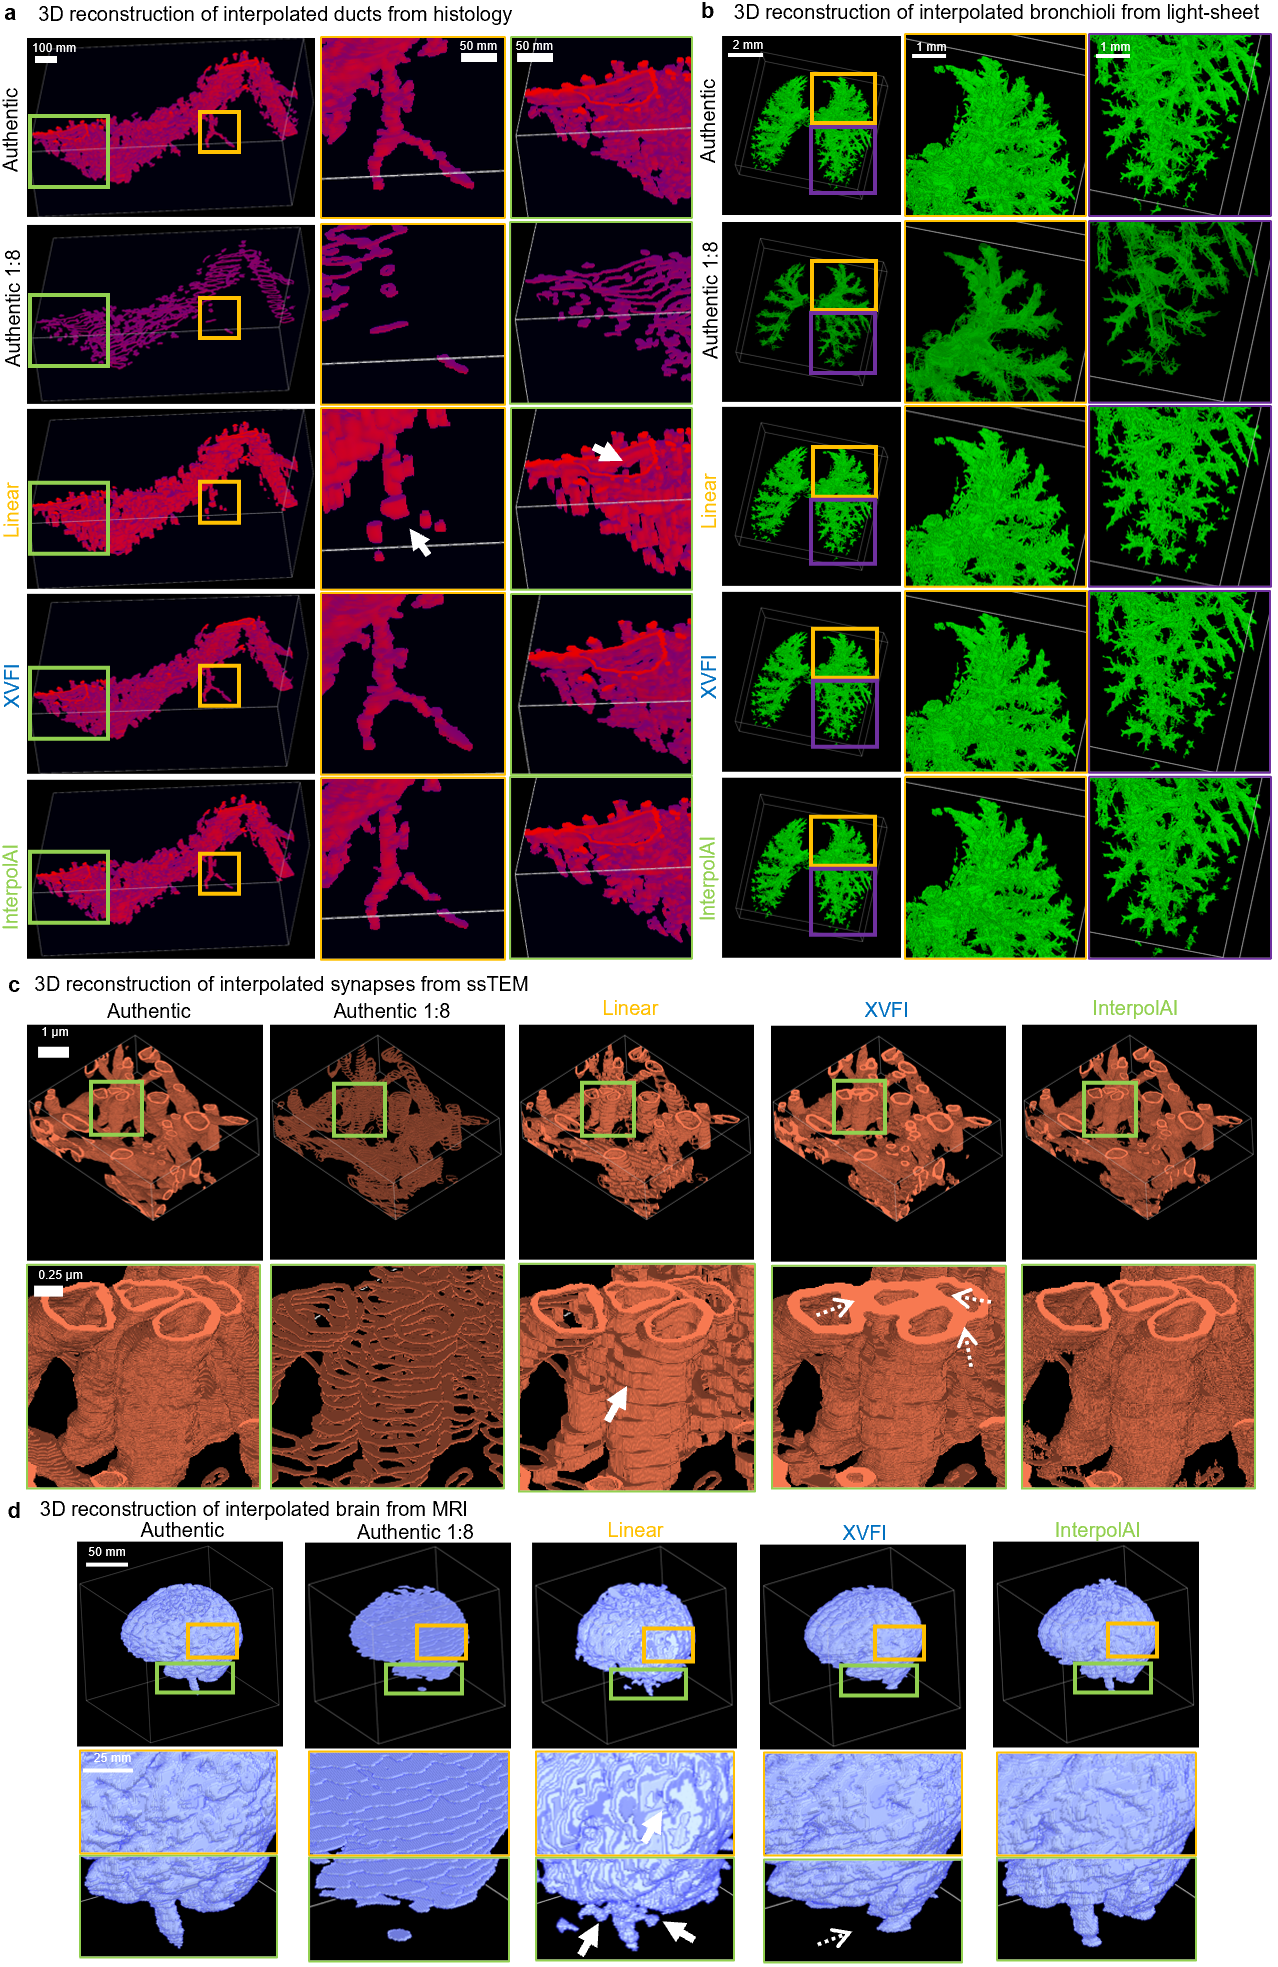
\includegraphics[width=\linewidth,                   height=0.85\textheight,                   keepaspectratio]{figures/chapter6/fig_6.png}
      \captionsetup{font=small}
      \caption{\textbf{3D reconstructions of interpolated images.} a, Comparison of 3D
        reconstructions of human pancreatic duct from a stack of H\&E sections, when
        skipping seven slides between authentic images and when interpolating the
        missing slides using linear, XVFI and InterpolAI interpolations. b, Comparison
        of 3D reconstructions of bronchioles from light-sheet images of the mouse lung
        when skipping seven images between authentic images and when interpolating
        the missing slides using linear, XVFI and InterpolAI interpolations.}
      \label{chapter6_fig6}
    \end{figure}
    
    \begin{figure}[h!]
        \ContinuedFloat
        \captionsetup{font=small}
        \caption[]{ c, Comparison
        of 3D reconstructions of synapses from ssTEM slides of the mouse brain when
        skipping seven images between authentic images and when interpolating the
        missing slides using linear, XVFI and InterpolAI interpolations. d, Comparison
        of 3D reconstructions of brain MRI images when skipping seven images between
        authentic images and when interpolating the missing slides using linear, XVFI and
        InterpolAI interpolations.}
    \end{figure}
    
    \section{Discussion}
    3D imaging of biomedical samples has become a requirement as 2D assessments are not sufficient in capturing the content and morphology of multi-cellular structures, rare events, and spatial relationships among different cell types.1 A multitude of platforms have been developed to leverage 2D biomedical stacks of histological, ssTEM, and tissue-cleared light-sheet images to reconstruct volumes of microanatomical structures and whole organs. Such platforms are highly dependent on the quality of individual 2D images within the image stacks for accurate volumetric reconstructions. Additionally, limitations in z-resolution of these 3D platforms often arise due to missing slides, tissue damage, and the high cost associated with 3D imaging. 
    Here, we address these challenges by introducing InterpolAI and its ability to extract and track features in biomedical images using optical flow for image interpolation. By interpolating between undamaged slides to recover missing or damaged slides, we bridge gaps in z-resolution. This workflow restores the connectivity of continuous microanatomical structures, such as ducts and blood vessels, in the 3D reconstructions and mitigates issues arising from damaged or missing slides. This method improves 2D biomedical image stacks for 3D reconstructions, subsequently improving quantitative assessments of cellular composition, tissue topography, and degree of branching of continuous structures.
    We conducted a thorough comparative assessment of the InterpolAI platform to linear and XVFI interpolation methods using thirteen Haralick texture features. Linear interpolation, which averages pixel intensities that create hued colors and structures, cannot create realistic biomedical images. As the number of images skipped increases, linearly interpolated images further degrade in authenticity, especially for the images furthest from the input images (middle-interpolated image). For large number of skipped images (e.g. skip 7), the middle-interpolated image presents strong hues as pixel intensities deviate largely between input images. XVFI interpolation, on the other hand, could more accurately generate synthetic biomedical images than linear interpolation, however XVFI was unable to achieve cellular resolution and was often limited in its ability to restore damage in images. Conversely, InterpolAI can interpolate biomedical images that resemble their authentic counterparts. 
    For light-sheet microscopy, InterpolAI accurately interpolates images in the z-direction reducing required z-steps during image acquisition. This significantly decreases imaging times of an entire sample, as imaging patterns are often imaged tile by tile laterally before moving to the next z-level. Collection time increases exponentially with the lateral size of the sample, from minutes for a 104 µm3 sample at a spatial resolution of 500 nm to a week for a 108 µm3 sample at the same resolution.16 InterpolAI interpolation helps address this limitation. 
    InterpolAI has a few limitations, which must be considered for optimal interpolation results. Firstly, InterpolAI requires well-aligned images for optimal interpolation. Using misaligned images leads to model hallucinations, which appear as unrealistic biological structures (Supplemental Figure \ref{chapter6_figS1}). InterpolAI handle vertical and horizontal misalignments well, up to a misalignment distance of 200 µm. However, InterpolAI cannot successfully interpolate images when they are bi-directionally or diagonally misaligned beyond a distance of 200 µm or rotated beyond 2°. Secondly, InterpolAI performs best when using non-damaged images as input pairs, which can result in the damage being propagated across the interpolated images. This is shown in the damage assessment carried out in Supplemental Figure \ref{chapter6_figS2}b and \ref{chapter6_figS2}f where positive data (+ y-axis) points show damage being propagated in interpolated images as a result of damaged inputs and negative data (− y-axis) points show damage being restored. Aside from obvious damage in input images such as tissue folds and tears, stain inconsistencies are an important consideration as sudden changes in pixel intensity and illumination between input images can cause model hallucinations. Lastly, InterpolAI generates images based on the two input images provided and therefore cannot predict rare events, which did not occur on either of the input images. This is also noticeable from the results obtained using the MRI dataset with thicker slices (1mm) as compared to thinly sliced ssTEM, tissue-cleared lightsheet microscopy, and histology images (8nm, 2μm). InterpolAI could not accurately predict large structural changes in MRI images when skipping 7 slides (8mm).
    In conclusion, our work goes beyond existing methods of image translation, such as CycleGANs and diffusion models that translate the same respective biomedical images from one image domain to another. Whereas image translation would require physical access to the slides of interest to be translated, our workflow interpolates missing, inaccessible, or damaged images, eliminates stitching artifacts, and works across diverse multimodal biomedical images .
    
    \begin{figure}[p] 
      \centering
      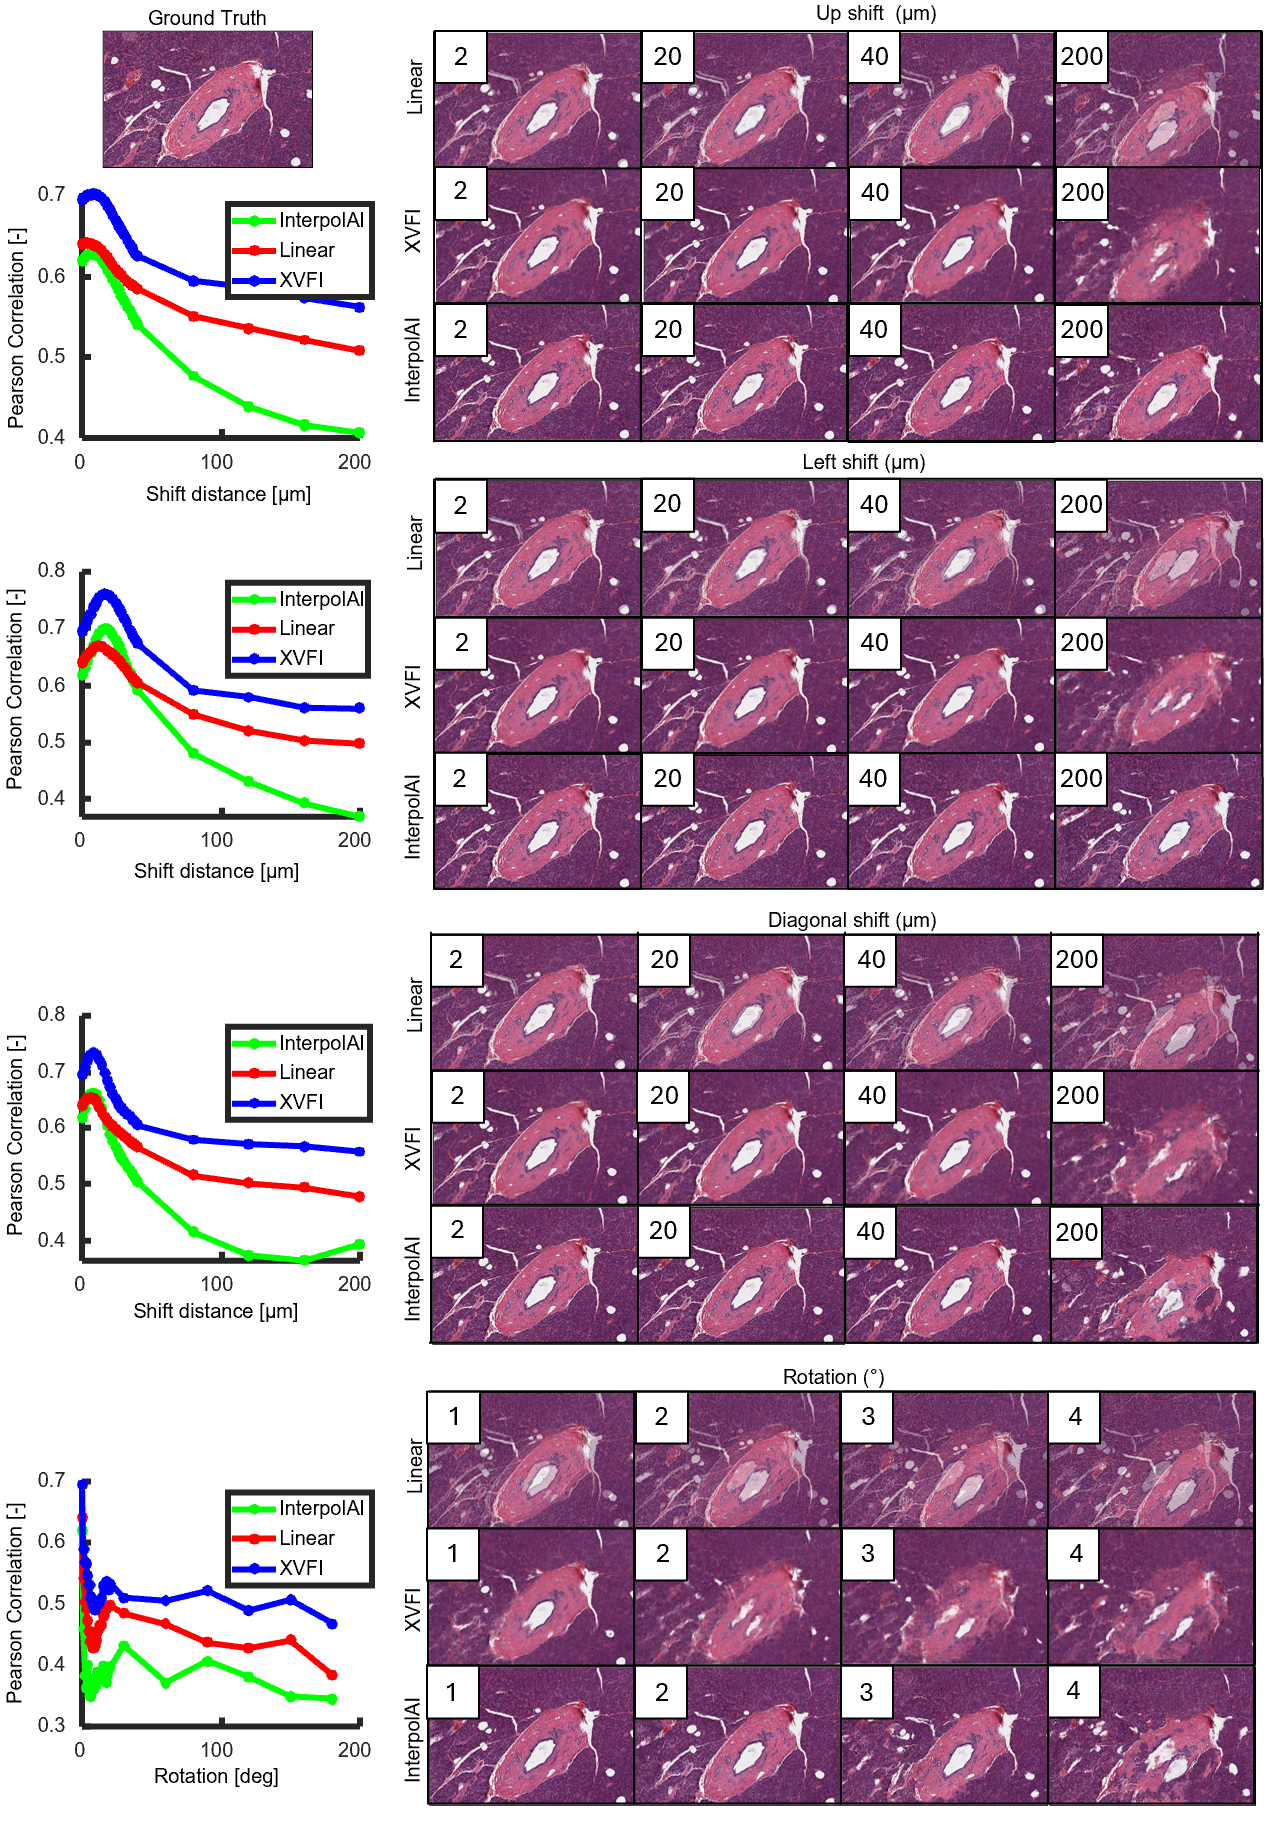
\includegraphics[width=\linewidth,                   height=0.85\textheight,                   keepaspectratio]{figures/chapter6/fig_S1.png}
      \captionsetup{font=small}
      \caption{\textbf{Effect of input image registration on the quality of interpolation.} (a) Simulated vertical misalignment of input images from 2-200μm misalignment and qualitative comparison of middle interpolated image to authentic image for all three methods of interpolation. Quantitative comparison of middle interpolated image to authentic image using Pearson correlation. }
      \label{chapter6_figS1}
    \end{figure}
    
    \begin{figure}[h!]
        \ContinuedFloat
        \captionsetup{font=small}
        \caption[]{ (b) Horizontal misalignment of input images from 2-200μm misalignment and qualitative comparison of middle interpolated image to authentic image for all three methods of interpolation. Quantitative comparison of middle interpolated image to ground truth using Pearson correlation. (c) Diagonal misalignment of input images from 2-200μm misalignment and qualitative comparison of middle interpolated image to authentic image for all three methods of interpolation. Quantitative comparison of middle interpolated image to authentic image using Pearson correlation. (b) Rotational misalignment of input images from 2-200° misalignment and qualitative comparison of middle interpolated image to authentic image for all three methods of interpolation. Quantitative comparison of middle interpolated image to authentic image using Pearson correlation.}
    \end{figure}

    \begin{figure}[p] 
      \centering
      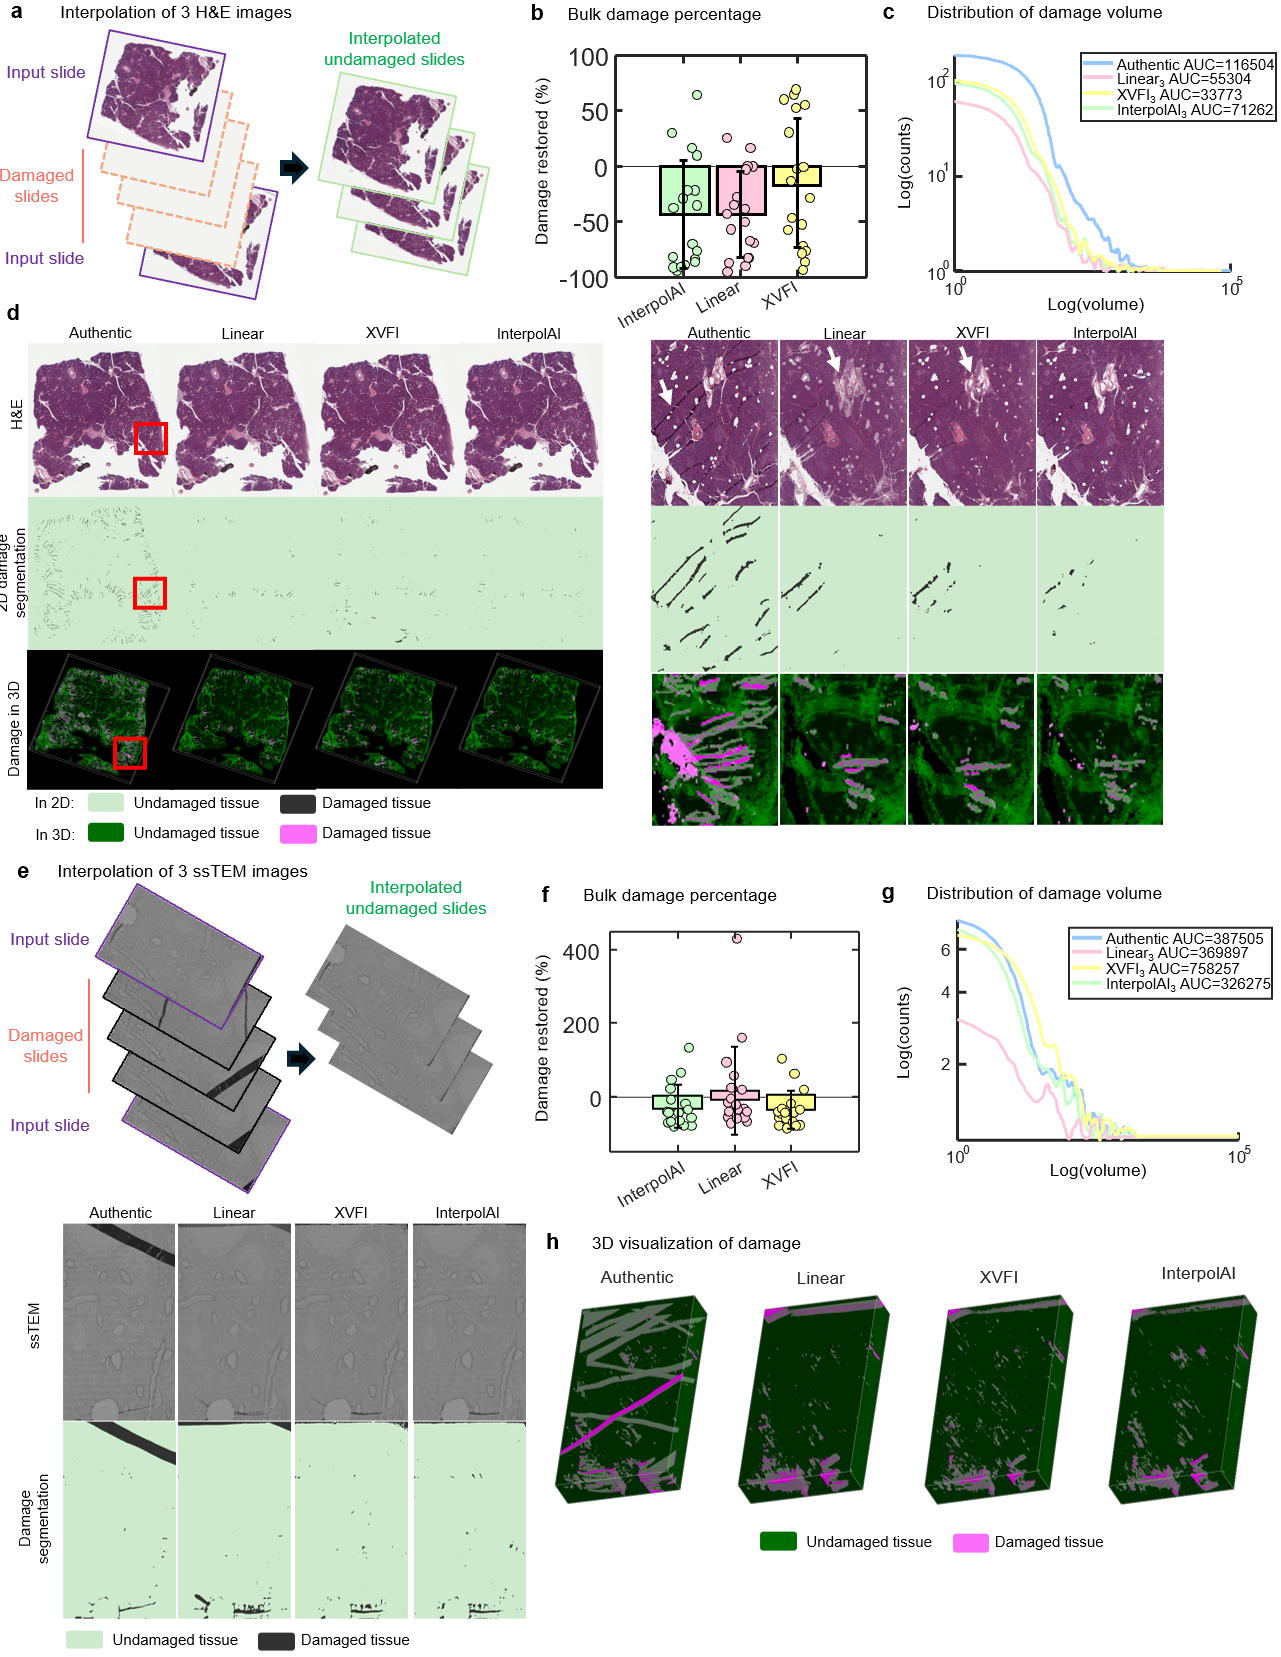
\includegraphics[width=\linewidth,                   height=0.85\textheight,                   keepaspectratio]{figures/chapter6/fig_S2.png}
      \captionsetup{font=small}
      \caption{\textbf{Assessment and effect of input image damage on the quality of interpolation. }(a) Subset of 25 consecutive slides from the H\&E histology dataset was selected and interpolated skipping 3 slides between adjacent sections.}
      \label{chapter6_figS2}
    \end{figure}
    
    \begin{figure}[h!]
        \ContinuedFloat
        \captionsetup{font=small}
        \caption[]{(b) CODA model was trained to detect folds in the H\&E histology dataset. Authentic WSIs and corresponding interpolated images were segmented into damaged and non-damaged labels. The percent difference in the number of damaged pixels for each pair of authentic and interpolated image was calculated. Positive data points (+ y-axis) demonstrate damage being propagated during interpolation as a result of picking damaged inputs, while negative data points (− y-axis) demonstrate damage being reduced with interpolation. (c) Log-log plot correlating damaged pixels on individual 2D slides with volumetric damage in 3D to showed damage reduction in both 2D and 3D as a result of the interpolation. (d) Comparison of middle interpolated H\&E to authentic for all 3 types of interpolation. CODA segmented damage/non-damage mask in 2D and 3D reconstructed damage/non-damage volume for authentic images and each interpolation method. Right panel shows zoom-in location boxed in red in left panel. (e) Subset of 25 consecutive slides from the ssTEM dataset was selected and interpolated skipping 3 slides between adjacent sections. (f) CODA model was trained to detect folded damage. Authentic and corresponding interpolated images were segmented into damaged and non-damaged labels. The percent difference in the number of damaged pixels for each pair of authentic and interpolated image was calculated and plotted. Positive data points (+ y-axis) demonstrate damage being propagated during interpolation as a result of picking damaged inputs, while negative data points (− y-axis) demonstrate damage being reduced with interpolation. (g) Log-log plot correlating damaged pixels on individual 2D slides with volumetric damage in 3D to show how damage is reduced in both 2D and 3D as a result of the interpolation. (h) Comparison of middle interpolated ssTEM image to authentic for all 3 types of interpolation. CODA segmented damage/non-damage mask in 2D and 3D reconstructed damage/non-damage volume for authentic images and each interpolation method.}
    \end{figure}
    
    \section{Materials and methods}
    \subsection{Specimen acquisition}
    A sample of non-diseased human pancreas tissue was stained with hematoxylin and eosin (denoted H\&E); another similar sample was stained with leukocyte marker CD45 via immunohistochemistry (denoted IHC-CD45). Both samples were from individuals who underwent surgical resection for pancreatic cancer at the Johns Hopkins Hospital.2 The H\&E dataset consisted of a stack of 101 serially sectioned slides at a resolution of 2µm x 2µm x 4µm. H and E are standard histological stains that mark nuclei and cellular structures (H) and ECM (E), respectively. The IHC-CD45 dataset consisted of 275 consecutive slides where every third section (16µm apart) was stained, at a resolution of 2µm x 2µm x 16µm and are described in Kiemen et al.\cite{kiemen2024a} CD45 is a general marker for leukocytes. This retrospective study was approved by the Johns Hopkins University Institutional Review Board (IRB).
    A stack of serial section transmission electron micrographs (ssTEM) within a densely annotated mouse visual cortex petascale image volume (public dataset Minnie65) was obtained through the online Brain Observatory Storage Service and Database (BossDB), created, and managed by the Johns Hopkins Applied Physics Laboratory (APL). This dataset consisted of 100 ssTEM slides captured at a resolution of 8nm x 8nm x 40nm.2,7
    Light-sheet microscopy images of mouse lung were obtained from the Image Data Resource (IDR) public repository.\cite{williams2017a,kubota2021a} This dataset consisted of 401 serial light-sheet microscopy images captured at a resolution of 3.22µm x 3.22µm x 10µm.
    MRI samples of human brain were obtained from the Amsterdam Open MRI Collection (AOMIC)\cite{snoek2021a}. Specifically, the PIOP2 (Population Imaging of Psychology) cohort consisting of structural MRI scans of students was used. The dataset consisted of 220 structural MRI scans captured at a resolution of 1mm x 1mm x 1mm. 
    
    \subsection{Segmentation of pancreatic microanatomy in histology slides}
    The previously developed semantic segmentation model CODA was leveraged to segment whole slide images (WSIs) of H\&E-stained pancreas samples into their different microanatomical components\cite{kiemen2022a,Crawford2024Combined,Braxton20243D}. CODA was specifically trained for the segmentation of microanatomical components of the pancreas and labeled seven components at a resolution of 2 µm per pixel, including islets of Langerhans, ductal epithelium, blood vessels, fat, acini, extracellular matrix (ECM), and pancreatic intraepithelial neoplasia (PanIN), which are precursor lesions of pancreatic cancer.2
    
    \subsection{Interpolation between 2D images}
    Spatial interpolation between 2D slides within a stack was carried out by developing InterpolAI, which is based on Frame Interpolation for Large Image Motion (FILM), a model previously developed for temporal interpolation between frames of videos by Reda et al.34 The model uses a three-step process to interpolate intermediate frames between two input images: a feature extraction pyramid, optical flow estimation, and feature fusion and frame synthesis. 
    The feature extraction pyramid consists of six convolutional layers responsible for extracting features from the input images, each with increasing kernel size and decreasing stride capturing progressively larger receptive fields, extracting features from coarser to finer scales. This coupled with the use of shared weights across scales, allows the model to extract features for both small and large motions efficiently.
    The features extracted are then fed into a bidirectional optical flow estimation module. This module calculates the pixel-wise motion vectors (or "flows") between the features of two input images at each pyramid level. These flows represent the transformation needed to warp the features from one frame to the other. The bi-directional approach allows the model to capture both forward and backward motion, leading to more accurate and detailed interpolations.34
    With the extracted features and estimated flows, FILM enters the final fusion stage. The aligned features from both input images, along with the flows and the original input images themselves, are concatenated into a single feature pyramid. This captures both the feature information and the motion dynamics between the two frames. Finally, a U-Net decoder architecture processes this fused feature pyramid and synthesizes the final interpolated frame. The U-Net's skip connections, which bypass several layers within the network and concatenate their outputs directly with the outputs of later layers, ensures that the interpolated frame retains fine details and maintains consistency with the input images.34
    FILM used a recursive function (Eq.1) which accounted for the number of input frames, n, and the number of recursive passes over which the model would interpolate, k. This limited the number of frames that could be interpolated between the input images to be either one, four, seven, or fifteen frames (Eq.1).
    \begin{equation} 
    \label{chapter_6_eq1}
        f = 2^k (n - 1) - 1 \tag{Eq.~1}
    \end{equation}
    Recognizing the need for flexibility in skipping slides based on user requirements, a time series spanning from 0 to 1 was implemented in InterpolAI, with step sizes dynamically determined by the number of skipped slides. This approach generated time points corresponding to the skipped slides, facilitating variable frame interpolation between input pairs.
    InterpolAI was pretrained on the Vimeo-90k dataset, a largescale dataset of 89,800 high quality videos designed specifically to train models oriented towards video processing tasks such as frame interpolation, image denoising and resolution enhancement.34 The optical flow of this model is already robustly pretrained on a diverse set of videos with different moving objects, such as vehicles, people, and smaller features like cameras and soccer balls. Re-training of the model posed two challenges: a lack of documentation on retraining and perfectly registering histological slides to curate a training dataset. The focus of InterpolAI on optical flow means that the model is sensitive to misalignment in the training images, making histological slides an unfavorable dataset to retrain the optical flow model due to inherent variability in tissue preparation, staining intensities, and sectioning processes, which lead to unpredictable distortions and variations that complicate accurate spatial alignment of a stack of slides. 
    For large images such as those encountered in histology, InterpolAI provides a tile-and-stitch algorithm to efficiently handle computer memory limitations. Whole slide images are tiled to a user defined size of 1024 or 2048 padded tiles each with an x and y index. Tiled images with the same x and y index are then used as inputs to interpolate images. Once all tiles are interpolated for each tile pair, the tiles are stitched back together with the pad area removed for each respective interpolated z-slide. This ensures the robustness of InterpolAI for not only small but large images at high magnification.  
    Two versions of the InterpolAI code were developed, a validation code and an operation code. The validation code uses a skip-count algorithm such that the image being interpolated exists in the provided folder path but was simply skipped and generated similarly to how it is presented in this study. The validation code then computes the Haralick texture features of both the skipped authentic image and the respective interpolated image. All Haralick scores are saved into csv file from which PCA analysis can be carried out. The operation code has a skip-count algorithm that generates images between each image pair in the provided folder path without skipping any image, thereby generating missing images. 
    
    \subsection{Registration assessment}
    To understand and quantify the alignment needed for image interpolation, the H&E dataset was used. Four different types of misalignments were considered, including a vertical shift, horizontal shift, diagonal shift, and rotation (Supplemental Fig. \ref{chapter6_figS1}). Using aligned slides at z = 31 and 33 from the H\&E dataset, a 3024x3024 tile was cropped from both whole slide images at the same position. For shift misalignment, the 3024x3024 tile from slide 31 was shifted horizontally, vertically, and diagonally from 0-200µm and then cropped to a 1024x1024 tile from the center, whereas slide 33 was left unshifted and cropped to a 1024x1024 tile from the center of the 3024x3024 tile. For rotation misalignment, the 3024x3024 tile from slide 31 was rotated 0 to 200 degrees from its center and then cropped to a 1024x1024 tile from the center, while slide 33 was left unrotated and cropped to a 1024x1024 tile from the center of the 3024x3024 tile. At a resolution of 2µm x 2µm x 4µm a 1-degree rotation from the center of a 3024x3024 tile corresponds to a 75µm misalignment at the furthest edges from the center of a 1024x1024 tile, as shown below: 
    
    \begin{equation}
    \label{chapter6_img_center}
        \textit{Image}_{\text{center}} = \left( \frac{3024}{2}, \frac{3024}{2} \right) = (1512, 1512)
    \end{equation}
    
    Considering the misalignment of the furthest point from the center, the distance from the center to the corner (R) is given by:
    \begin{equation}
        R = \sqrt{(1512)^2 + (1512)^2} = 2138.6 \, \text{pixels}
    \end{equation}
    
    \begin{equation}
        R_{\mu\text{m}} = 2138.6 \, \text{pixels} \times 2 \, \mu\text{m/pixel} = 4277.2 \, \mu\text{m}
    \end{equation}
    Using arc length formula (Eq. 2) the maximum displacement (Δs) at the edge furthest from the center of the image can be calculated as:
   \begin{equation}
   \label{chapter_6_eq2}
        \Delta s = R_{\mu\text{m}} \cdot \theta \tag{Eq.~2}
    \end{equation}
    Calculating for a rotation of 1 degree:
    \begin{equation}
        \theta = \frac{1 \times \pi}{180} = 0.01745 \, \text{radians}
    \end{equation}
    
    \begin{equation}
        \Delta s = 4277.2 \, \mu\text{m} \times 0.01745 = 74.6 \, \mu\text{m}
    \end{equation}
    Interpolation using InterpolAI, linear interpolation and XVFI was conducted between shifted and rotated slide 31 and unchanged slide 33 to generate slide 32, which was then correlated to the authentic slide 32 using Pearson correlation. The Pearson correlation was calculated using the SciPy stats package available in python.  
    
    \subsection{Haralick texture features}
    Thirteen Haralick texture features were calculated to provide a quantitative representation of the texture patterns within an image, offering insights into their spatial arrangements and relationships\cite{brynolfsson2017a,haralick1973a}. The 13 features measure the angular second moment, contrast, correlation, sum of squares variance, inverse difference moment, sum average, sum variance, difference variance, sum entropy, difference entropy, entropy, information measure of correlation 1, and information measure of correlation 2\cite{brynolfsson2017a,haralick1973a}. Contrast measures the intensity variations between neighboring pixels, correlation gauges the linear dependency of gray levels, energy represents the image uniformity, and homogeneity measures the closeness of gray level pairs.
    To manage the complexity and high dimensionality of the feature space, dimensionality reduction was carried out using principal component analysis (PCA). PCA transformed the original set of Haralick features into a reduced set of principal components, retaining the most significant information while discarding redundant or less informative aspects. This reduction not only simplifies the interpretation of the data, but also allows for a holistic assessment of image quality, capturing the essential texture information in a more compact form.
    Additionally, analysis of the Euclidean distances between authentic and interpolated images was computed using the 13 Haralick features. By considering the Euclidean distances across all selected Haralick features simultaneously, a comprehensive evaluation of the overall error value was achieved. This validation process ensured that the collective impact of texture features was considered, providing a robust measure of similarity/dissimilarity between images. The combination of Haralick texture features, PCA for dimensionality reduction, and Euclidean distance computation offered a systematic and effective approach for evaluating image quality and texture patterns.
    Cell detection in histological sections
    To validate the (synthetic) interpolated H&E and IHC images, the CODA cell detection module was used to count the total number of cells in H&E images and CD45+ cells in IHC and compare these numbers with those in their respective authentic images.2 For this task, the intensity range of blue pixels was first determined for the nuclei of cells, along with the intensity of brown pixels for positive CD45 stain. Using k-means clustering, the mode blue pixel intensity was determined and selected to represent the hematoxylin channel, while the mode brown pixel intensity was selected to represent the positive stain. With color deconvolution, the cells stained with hematoxylin could be extracted from the remaining tissue, thereby providing a cell count.
    
    \subsection{Quantification of damage }
    To understand and quantify the quality of input images required for image interpolation, a damage assessment was carried out on a subset of the last 25 consecutive slides from the H&E data set and 25 images of the ssTEM dataset (Supplemental Fig. \ref{chapter6_figS2}). A CODA segmentation model was trained to detect folds in both datasets and segment them as damage. Next, interpolation of both datasets was carried out while skipping 3 authentic images and interpolating them. The interpolated images were subsequently segmented using the same CODA segmentation model to detect folds as was done with the authentic images. Using the segmented images, the difference in the total number of folded pixels between the interpolated images and authentic images was determined and divided by the total number of folded pixels in the authentic images to determine the percent by which damaged was reduced through interpolation (Supplemental Fig. \ref{chapter6_figS2}b and 2f). Segmented images were also used to plot the folds in both datasets in 3D and show the reduction in folds through interpolation. The number of folded pixels in individual 2D images were plotted against the size of the fold in 3D to obtain a log-log plot of the reduction in folds in 3D, as a result of interpolation (Supplemental Fig. \ref{chapter6_figS2}c and 2g)
    
    \subsection{3D rendering of interpolated 2D images}
    InterpolAI was used to interpolate stacks of whole slide images (WSIs) of missing or damaged slides, which resulted in a whole restored dataset (Fig. \ref{chapter6_fig1}b). For image post-processing, CODA was used to semantically segment histological slides and MRI images to reconstruct microanatomical tissue structures and whole organs in 3D (Fig. \ref{chapter6_fig1}b). Through manual annotations of microanatomical tissue structures in a small subset of histology slides and whole organ annotations of the brain in a subset of MRI images, CODA allowed for two deep learning models to be trained to recognize these annotations and apply them to the remaining slides/images in the respective datasets, thereby generating stacks of segmented histology slides and MRI images. Labels within the segmented slides/images, corresponding to the annotations could then be used by CODA to reconstruct and visualize 3D tissue structures of interest, such as epithelial ducts in the pancreas, and whole organs such as the brain. Similarly, CODA was leveraged to 3D reconstruct synapses in the mouse brain using pre-segmented ssTEM slides with the appropriate synapse label. Tissue-cleared light-sheet images were separated into their respective RGB channels allowing for three stacks to be obtained, one for each channel. 3D reconstructions of structures within the tissue-cleared light-sheet images of the lung were then generated by creating volumes using stacks of channel-separated images. Specifically, the red channel was used to reconstruct the bronchioles in the mouse lung.
    
    \subsection{Computing hardware and software}
    We used Python (v3.9) and Tensorflow (2.10.0) for all image interpolations and analysis. For the CODA quantifications and 3D renderings, we used MATLAB (2023a).
    For smaller sized images, computers equipped with a single NVIDIA RTX 3090 GPU could easily interpolate them. For larger whole slide images, with dimensions exceeding 14,000x10,000 pixels, using more GPU power allowed to speed up the interpolation processing times. To handle these larger images with higher magnifications, we utilized the Rockfish cluster at Johns Hopkins University, which is equipped with nodes containing four NVIDIA A100 GPUs each. This high-performance computing resource enabled us to interpolate whole slide histological images in shorter times. In case of no access to GPU clusters, users may opt for a tile and stitch approach provided in our code, which allows for tiling of large WSIs, interpolating the tiles individually, and then stitching them back together into WSIs during post-processing. The codes and requirements for InterpolAI have been posted on GitHub.  
    
    \clearpage
    \printbibliography[heading=subbibliography, title={References}]
\end{refsection}